% Autor: Leonhard Segger, Alexander Neuwirth
% Datum: 2017-10-30
\documentclass[
	% Papierformat
	a4paper,
	% Schriftgröße (beliebige Größen mit „fontsize=Xpt“)
	12pt,
	% Schreibt die Papiergröße korrekt ins Ausgabedokument
	pagesize,
	% Sprache für z.B. Babel
	ngerman
]{scrartcl}

% Achtung: Die Reihenfolge der Pakete kann (leider) wichtig sein!
% Insbesondere sollten (so wie hier) babel, fontenc und inputenc (in dieser
% Reihenfolge) als Erstes und hyperref und cleveref (Reihenfolge auch hier
% beachten) als Letztes geladen werden!

% Silbentrennung etc.; Sprache wird durch Option bei \documentclass festgelegt
\usepackage{babel}
% Verwendung der Zeichentabelle T1 (Sonderzeichen etc.)
\usepackage[T1]{fontenc}
% Legt die Zeichenkodierung der Eingabedatei fest, z.B. UTF-8
\usepackage[utf8]{inputenc}
% Schriftart
\usepackage{lmodern}
% Zusätzliche Sonderzeichen
\usepackage{textcomp}

% Mathepaket (intlimits: Grenzen über/unter Integralzeichen)
\usepackage[intlimits]{amsmath}
% Ermöglicht die Nutzung von \SI{Zahl}{Einheit} u.a.
\usepackage{siunitx}
% Zum flexiblen Einbinden von Grafiken (\includegraphics)
\usepackage{graphicx}
% Abbildungen im Fließtext
\usepackage{wrapfig}
% Abbildungen nebeneinander (subfigure, subtable)
\usepackage{subcaption}
% Funktionen für Anführungszeichen
\usepackage{csquotes}
% Zitieren, Bibliographie
\usepackage{biblatex}

\usepackage{subcaption}


% Zur Darstellung von Webadressen
\usepackage{url}
%chemische Formeln
\usepackage[version=4]{mhchem}
% siunitx: Deutsche Ausgabe, Messfehler getrennt mit ± ausgeben
\usepackage{floatrow}
\floatsetup[table]{capposition=top}
\usepackage{float}
% Verlinkt Textstellen im PDF-Dokument
\usepackage[unicode]{hyperref}
% "Schlaue" Referenzen (nach hyperref laden!)
\usepackage{cleveref}
\sisetup{
	locale=DE,
	separate-uncertainty
}
\bibliography{14Mo_O7_23-04-2018_References}

\begin{document}
	
	\begin{titlepage}
		\centering
		{\scshape\LARGE Versuchsbericht zu \par}
		\vspace{1cm}
		{\scshape\huge O7 - Beugung am Spalt, Doppelspalt und Gitter \par}
		\vspace{2.5cm}
		{\LARGE Gruppe 14Mo \par}
		\vspace{0.5cm}
		
		{\large Alexander Neuwirth (E-Mail: a\_neuw01@wwu.de) \par}
		{\large Leonhard Segger (E-Mail: l\_segg03@uni-muenster.de) \par}
		\vfill
		
		durchgeführt am 23.04.2018\par
		betreut von\par
		{\large Lukas Britt}
		
		\vfill
		
		{\large \today\par}
	\end{titlepage}
	\tableofcontents
	\newpage

	\section{Kurzfassung}
	
	Es wurde mithilfe eines Aufbaus zur Erfassung der Intensitätsverteilung verschiedener Spaltanordnungen die Abhängigkeit des Intensitätsbildes von Spaltbreite, Spaltabstand und Spaltanzahl untersucht und mit der Theorie zu Einfach- und Mehrfachspalten verglichen.
	Daraus wurde auch die Wellenlänge des verwendeten Lasers und die Gitterstruktur bestimmt.
	Für die Wellenlänge des Laserlichts haben wir eine Wellenlänge von \SI{630}{\nano \meter} bis \SI{680}{\nano \meter} erwartet, da dies die Angabe auf dem Laser war.
	Dies wurde mit einem Messwert von \SI{663 \pm 11}{nm} bestätigt.
	Bei der Intensitätsverteilung eines Einzelspalts ist ein Verlauf gemäß der quadrierten sinc-Funktion zu erwarten gewesen und wurde auch so gemessen.
	Beim Doppelspalt erwarteten wir ein Intensitätsbild in Form einer Oszillation mit der Intensitätsverteilung des Einzelspalts mit selber Spaltbreite als einhüllende Funktion, was jedoch nicht eindeutig nachgewiesen werden konnte.
	Der Vergleich der Intensitätsverteilung von Doppelspalten mit verschiedenen Spaltabständen und Spaltbreiten hat sich, wie es die Theorie vorhersagt, verhalten (vgl. \cref{Doppelspalttheo}). 
	Außerdem erwarten wir bei Mehrfachspalten einen Anstieg der Intensität der Hauptmaxima mit der Anzahl der Spalte.
	Dies konnte für kleine Spaltzahlen bestätigt werden und die Gitterstruktur konnte bestimmt werden.
	Außerdem erwarteten wir einen quadratischen Zusammenhang zwischen Anzahl der Spalte eines Mehrfachspalts und Intensität der Hauptmaxima.
	
	\section{Methoden}
	In \cref{optischeBank} ist der Aufbau des Experiments illustriert.
	An einem Ende der optischen Bank befindet sich ein Diodenlaser und davor ein Polarisator und der Halter für Spalte.
	Am anderen Ende der optischen Bank ist eine durch eine Kurbel senkrecht zu optischen Bank zu bewegende Photodiode angebracht.
	Die Halterung der Photodiode ist über ein Seil mit einem Rad verbunden, um die Intensitätsmessung der Diode mit der Position der Diode im Strahlengang zu verbinden.
	Nun kann eine Spaltanordnung in die Halterung gebracht werden und durch Bewegung der Photodiode über die optische Bank die Intensitätsverteilung der Spalte bestimmt werden.
	Dabei wurde an den Rändern der Intensitätsverteilung mit kaum von Null verschiedener Beleuchtungsstärke weniger Messwerte aufgenommen als nahe der Mitte.
	Dies wurde realisiert durch unterschiedlich schnelle Bewegung der Photodiode bei konstanter Messfrequenz.
	Durch Veränderung der Empfindlichkeit der Diode und der Intensität des einfallenden Lichtstrahls durch den Polarisator, wurde der Messbereich der Photodiode möglichst vollständig ausgenutzt.
	In dieser Art und Weise wurden unterschiedliche Spaltanordnungen untersucht. 
	
	\begin{figure}[H]
		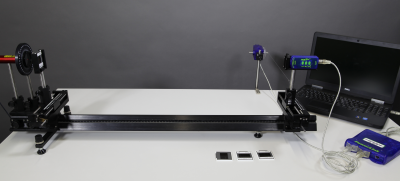
\includegraphics[width=0.7\textwidth]{optischeBank}
		\centering
		\caption{Aufbau der optischen Bank. Auf der linken Seite sind Laser und Beugungsanordnung und auf der rechten Seite die Photodiode zu sehen.\cite{optischeBank} }
		\label{optischeBank}
		\centering
	\end{figure} 
	
	\section{Ergebnisse und Diskussion}
	

	\subsection{Beobachtung}
	
	\subsubsection{Bestimmen der Wellenlänge des Laserlichts}
	In \crefrange{Einzelspalt0-075mm}{Einzelspalt0-400mm} sind für Einzelspalte der Breite $b$ = \SI{0,075}{mm}, \SI{0,15}{mm} und \SI{0,4}{mm} die Intensitätsverteilungen dargestellt. 
	Die Unsicherheit der Breite wird mit 1\% abgeschätzt.
	Mit \cref{einzelminmax} lässt sich aus der Positionen von einem Minimum ( $m$ = $\pm1$, $\pm 2$, ...) oder Maximum ( $m$ = $\pm\frac{3}{2}$, $\pm \frac{5}{2}$, ...) die Wellenlänge $\lambda$ berechnen. 
	
	\begin{equation}
		\sin(\vartheta) = m \frac{\lambda}{b}
		\label{einzelminmax}
	\end{equation}
	Der Winkel $\sin(\vartheta)$ ergibt sich nach \cref{dreieck} aus dem Abstand des Gitters zum Schirm bzw. Sensor $d$ = \SI{0,78 +- 0,009}{m} und der Position des Extremas $x$. 
	\begin{equation}
		\sin(\vartheta) = \frac{x}{\sqrt{d^2 + x^2}}
		\label{dreieck}
	\end{equation}
	Für die Wellenlänge folgt:
	\begin{equation}
		\lambda = \frac{b}{m\sqrt{(d/x)^2 + 1}}
	\end{equation}
	\begin{equation}
	u(\lambda) = \frac{\lambda}{d^2+x^2} \sqrt{\left( \frac{d^2}{x} u(x)\right)^2 + \left( \frac{(d^2+ x^2)}{b}u(b) \right) ^2 + \left( du(d) \right)^2}
	\end{equation}
	
	\begin{table}[H]
		\centering
		\begin{tabular}{ c | c | c | c }
			$b$ & $m$ &  $|x|$ & $\lambda$ \\ \hline
			\SI{0,075 +- 0,0008}{mm} & -1,5 & \SI{10 +- 0,2}{mm} & \SI{641 +- 16}{nm} \\
			\SI{0,075+- 0,0008}{mm} & -1,0 & \SI{7,5 +- 0,2}{mm} & \SI{673+-22}{nm} \\
			
			\SI{0,150+- 0,0015}{mm} & 1,5 & \SI{5 +- 0,2}{mm} & \SI{641+-27}{nm} \\
			\SI{0,150+- 0,0015}{mm} & 1,0 & \SI{4 +- 0,2}{mm} & \SI{770+-40}{nm} \\
			\SI{0,150+- 0,0015}{mm} & -1,5 & \SI{4,9 +- 0,2}{mm} & \SI{628+-27}{nm} \\
			\SI{0,150+- 0,0015}{mm} & -1,0 & \SI{3,5 +- 0,2}{mm} & \SI{673+-40}{nm} \\
			
			\SI{0,150+- 0,0015}{mm} & 2,5 & \SI{9 +- 0,2}{mm} & \SI{692+-19}{nm} \\
			\SI{0,150+- 0,0015}{mm} & 2,0 & \SI{7 +- 0,2}{mm} & \SI{673+-22}{nm} \\
			\SI{0,150+- 0,0015}{mm} & -2,5 & \SI{8 +- 0,2}{mm} & \SI{615+-18}{nm} \\
			\SI{0,150+- 0,0015}{mm} & -2,0 & \SI{7 +- 0,2}{mm} & \SI{673+-22}{nm} \\
			
			\SI{0,400+- 0,004}{mm} & 1,5 & \SI{1,8 +- 0,02}{mm} & \SI{615+-16}{nm} \\
			\SI{0,400+- 0,004}{mm} & 1,0 & \SI{1,3 +- 0,02}{mm} & \SI{667+-14}{nm} \\
			\SI{0,400+- 0,004}{mm} & -1,5 & \SI{1,9 +- 0,02}{mm} & \SI{650+-12}{nm} \\
			\SI{0,400+- 0,004}{mm} & -1,0 & \SI{1,3 +- 0,02}{mm} & \SI{667+-14}{nm} \\
		\end{tabular}
		\caption{Aus Extrema ermittelte Wellenlängen für verschiedene Spaltbreiten.}
		\label{Einzelspalte} 
	\end{table}
	Der Mittelwert der Wellenlängen aus \cref{Einzelspalte} beträgt $\bar{\lambda}$ = \SI{663 +- 11}{nm}.
	%TODO zu klein?!? => nicht in eine Zeile => ?ANHANG?
	\begin{figure}[H]
		\centering
		\begin{subfigure}{.5\textwidth}
			\centering
			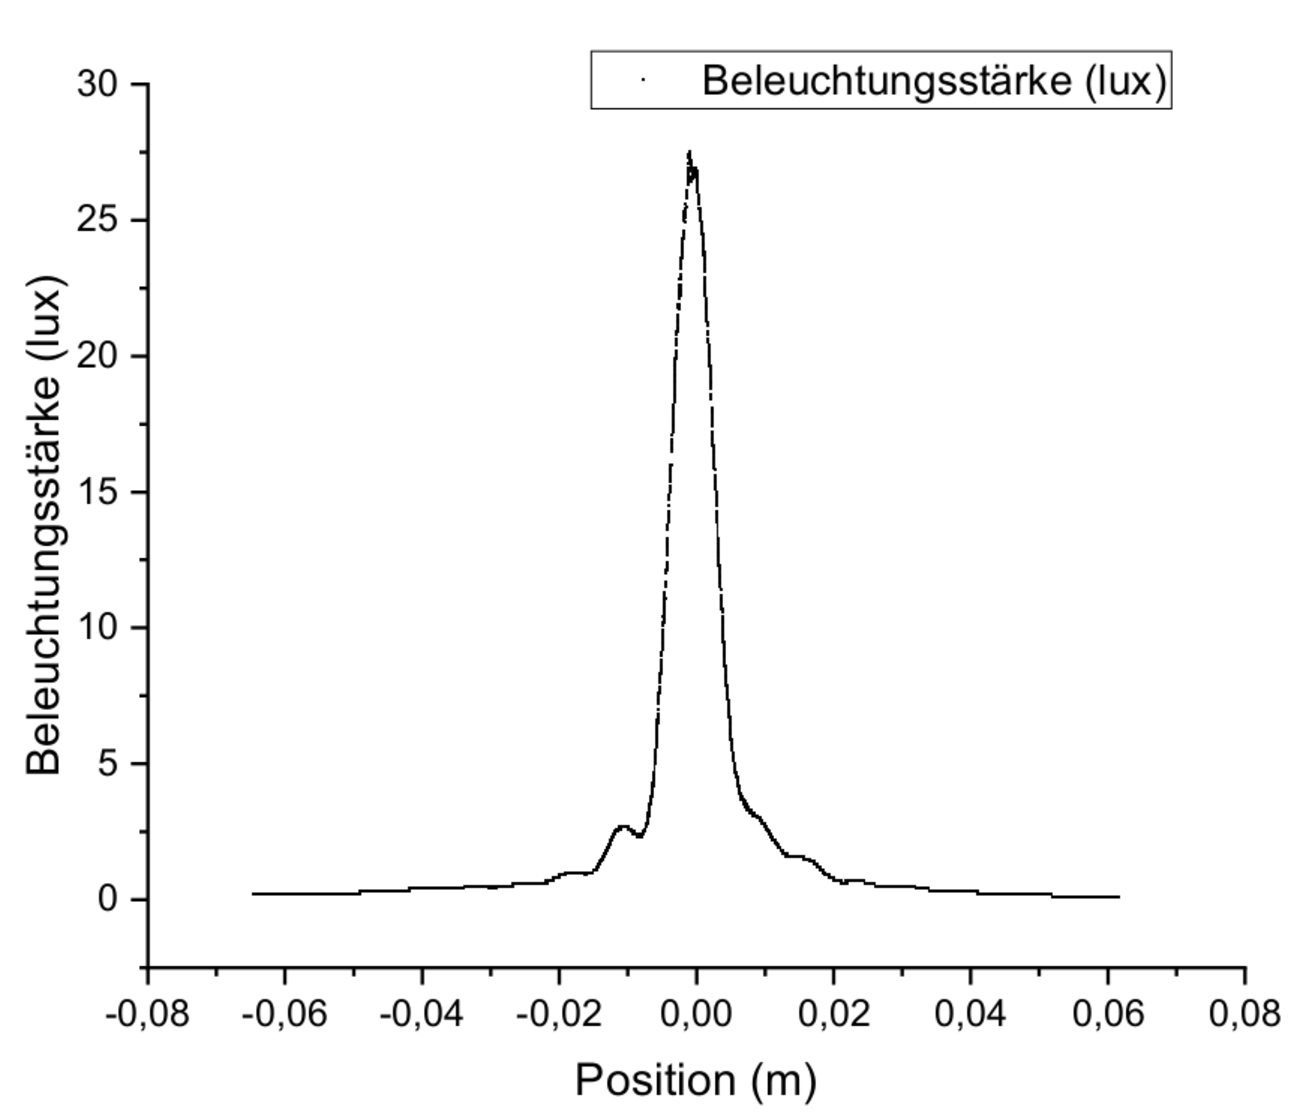
\includegraphics[width=1\linewidth]{Einzelspalt0-075mm}
			\caption{Gesamte Messung}	
		\end{subfigure}%
		\begin{subfigure}{.5\textwidth}
			\centering
			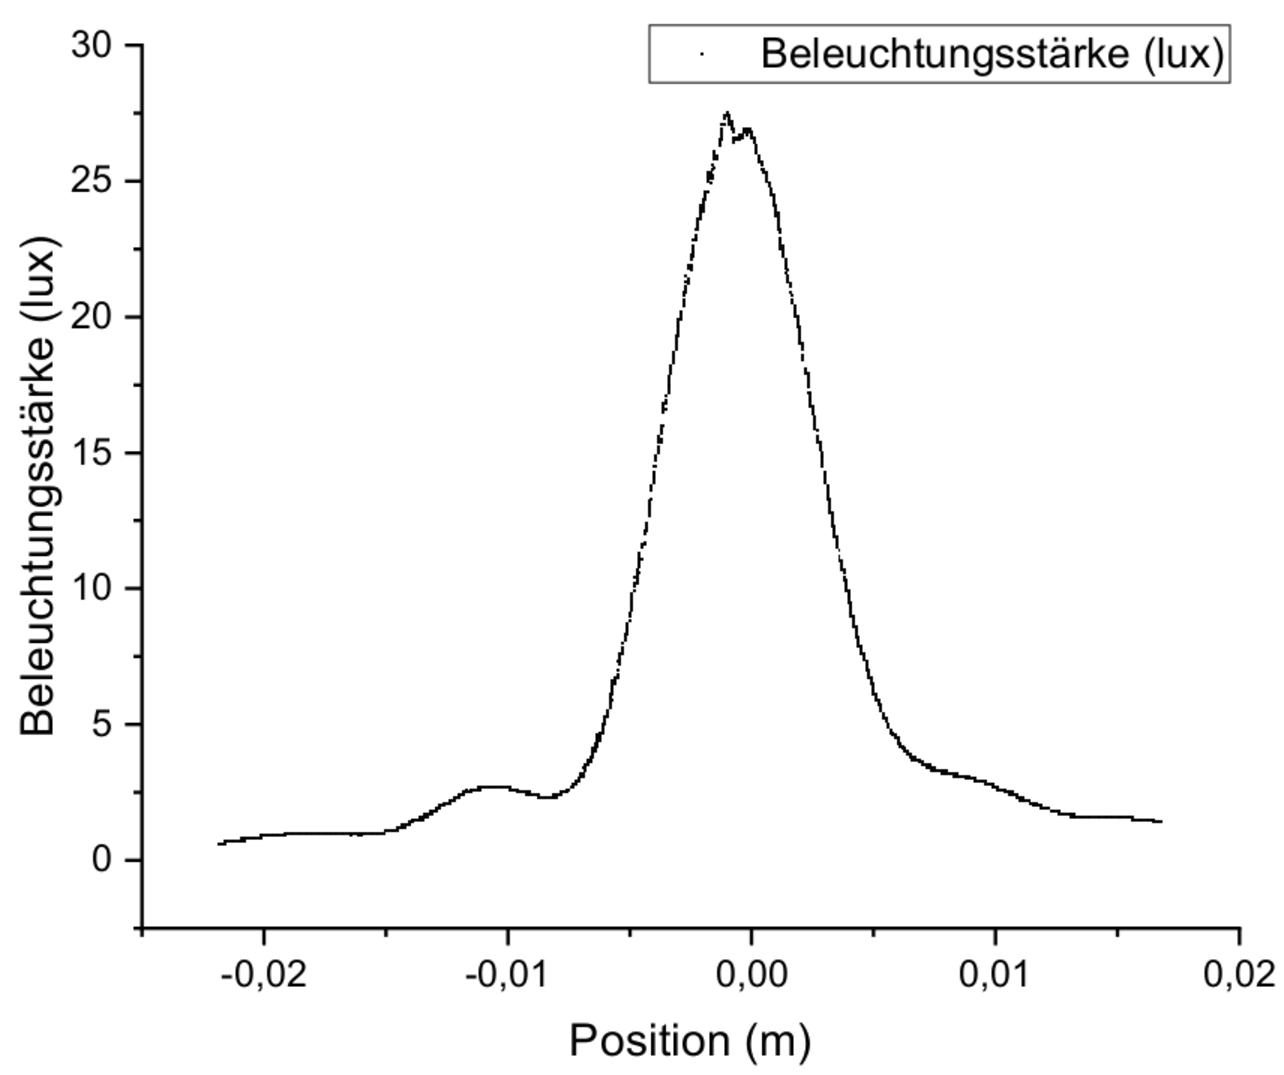
\includegraphics[width=1\linewidth]{Einzelspalt0-075mmZOOM}
			\caption{Extrema niedriger Ordnung}
		\end{subfigure}
		\caption{Intensitätsverteilung für einen Einzelspalt mit der Spaltbreite $b$ = \SI{0,075}{mm}.}
		\label{Einzelspalt0-075mm}
	\end{figure}	
	\begin{figure}[H]
		\centering
		\begin{subfigure}{.5\textwidth}
			\centering
			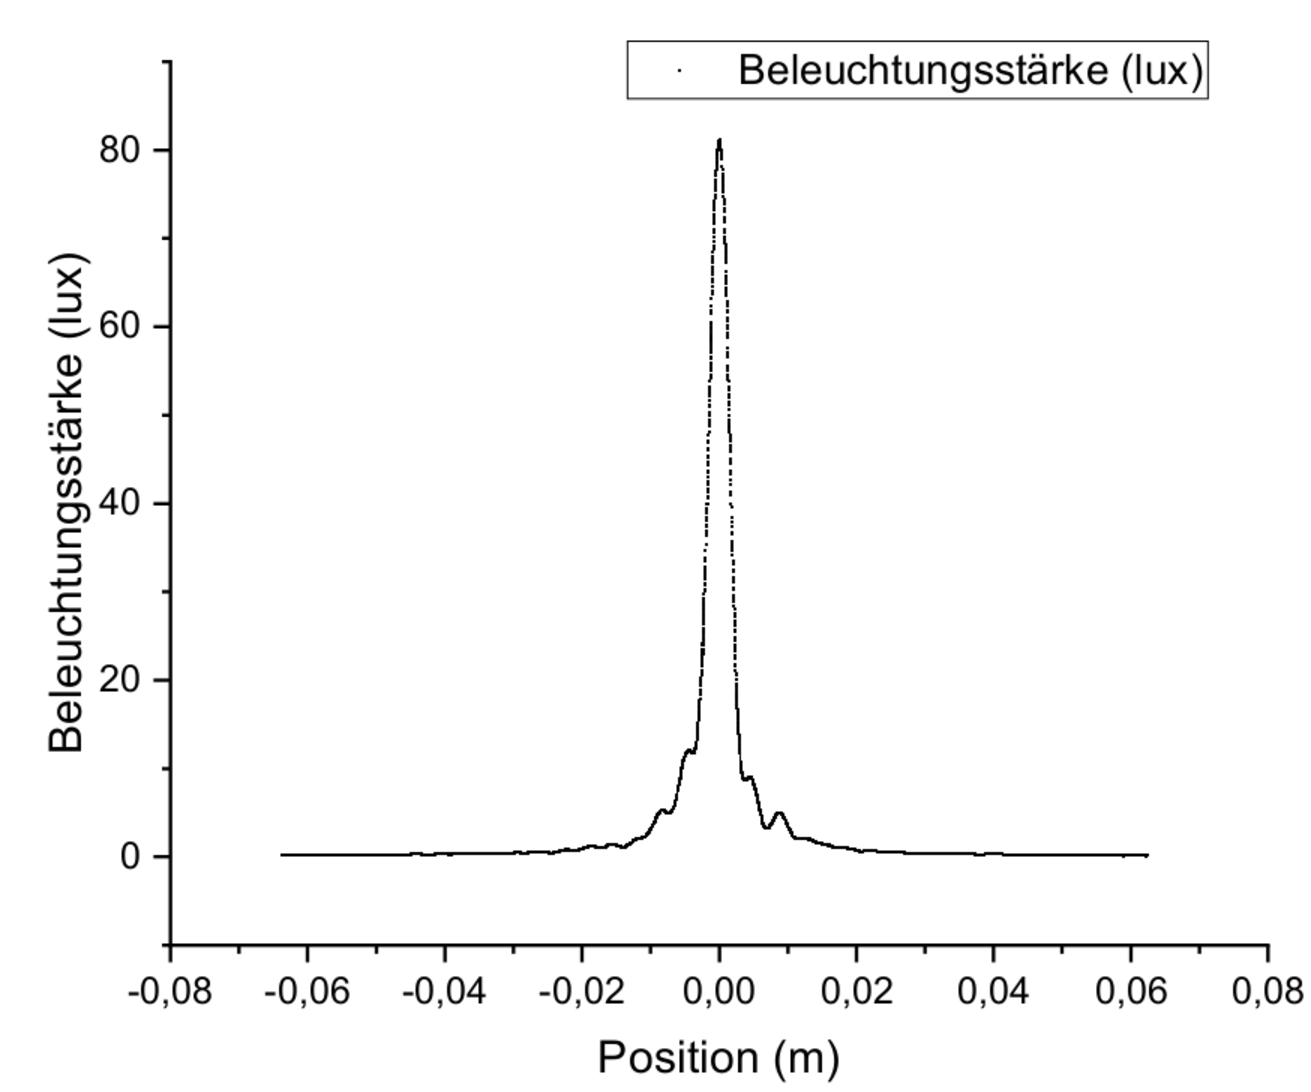
\includegraphics[width=1\linewidth]{Einzelspalt0-150mm}
			\caption{Gesamte Messung}	
		\end{subfigure}%
		\begin{subfigure}{.5\textwidth}
			\centering
			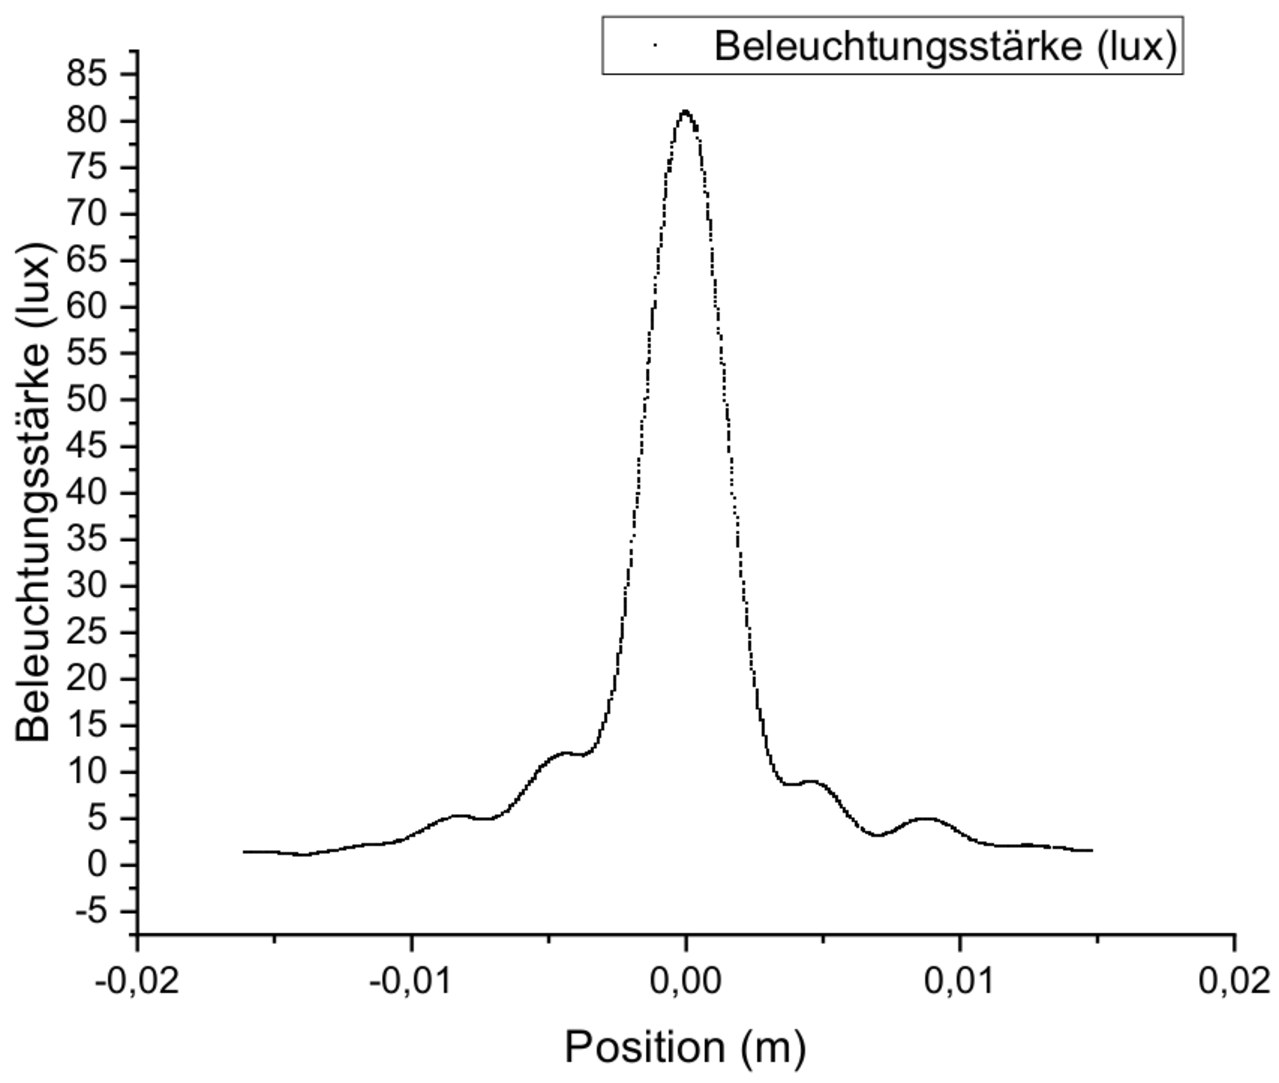
\includegraphics[width=1\linewidth]{Einzelspalt0-150mmZOOM}
			\caption{Extrema niedriger Ordnung}
		\end{subfigure}
		\caption{Intensitätsverteilung für einen Einzelspalt mit der Spaltbreite $b$ = \SI{0,15}{mm}.}
		\label{Einzelspalt0-150mm}

	\end{figure}	

	\begin{figure}[H]
		\centering
		\begin{subfigure}{.5\textwidth}
			\centering
			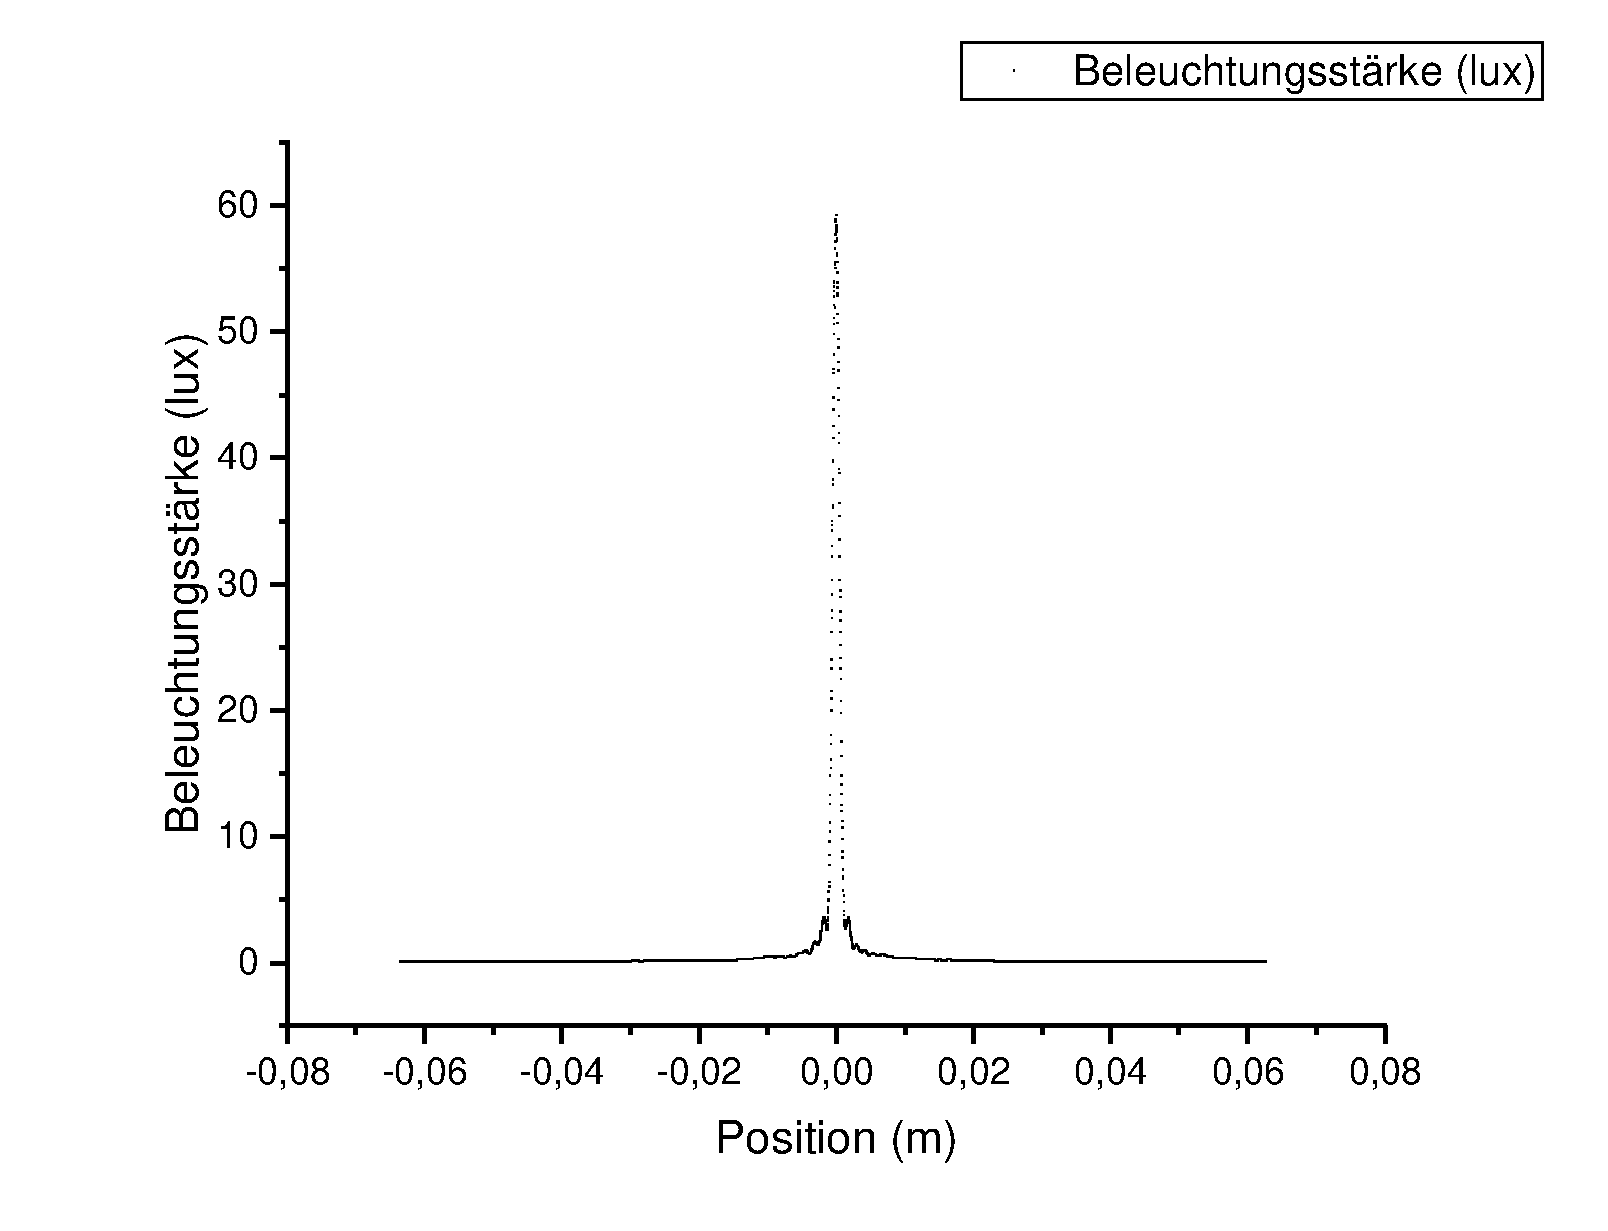
\includegraphics[width=1\linewidth]{Einzelspalt0-400mm}
			\caption{Gesamte Messung}	
		\end{subfigure}%
		\begin{subfigure}{.5\textwidth}
			\centering
			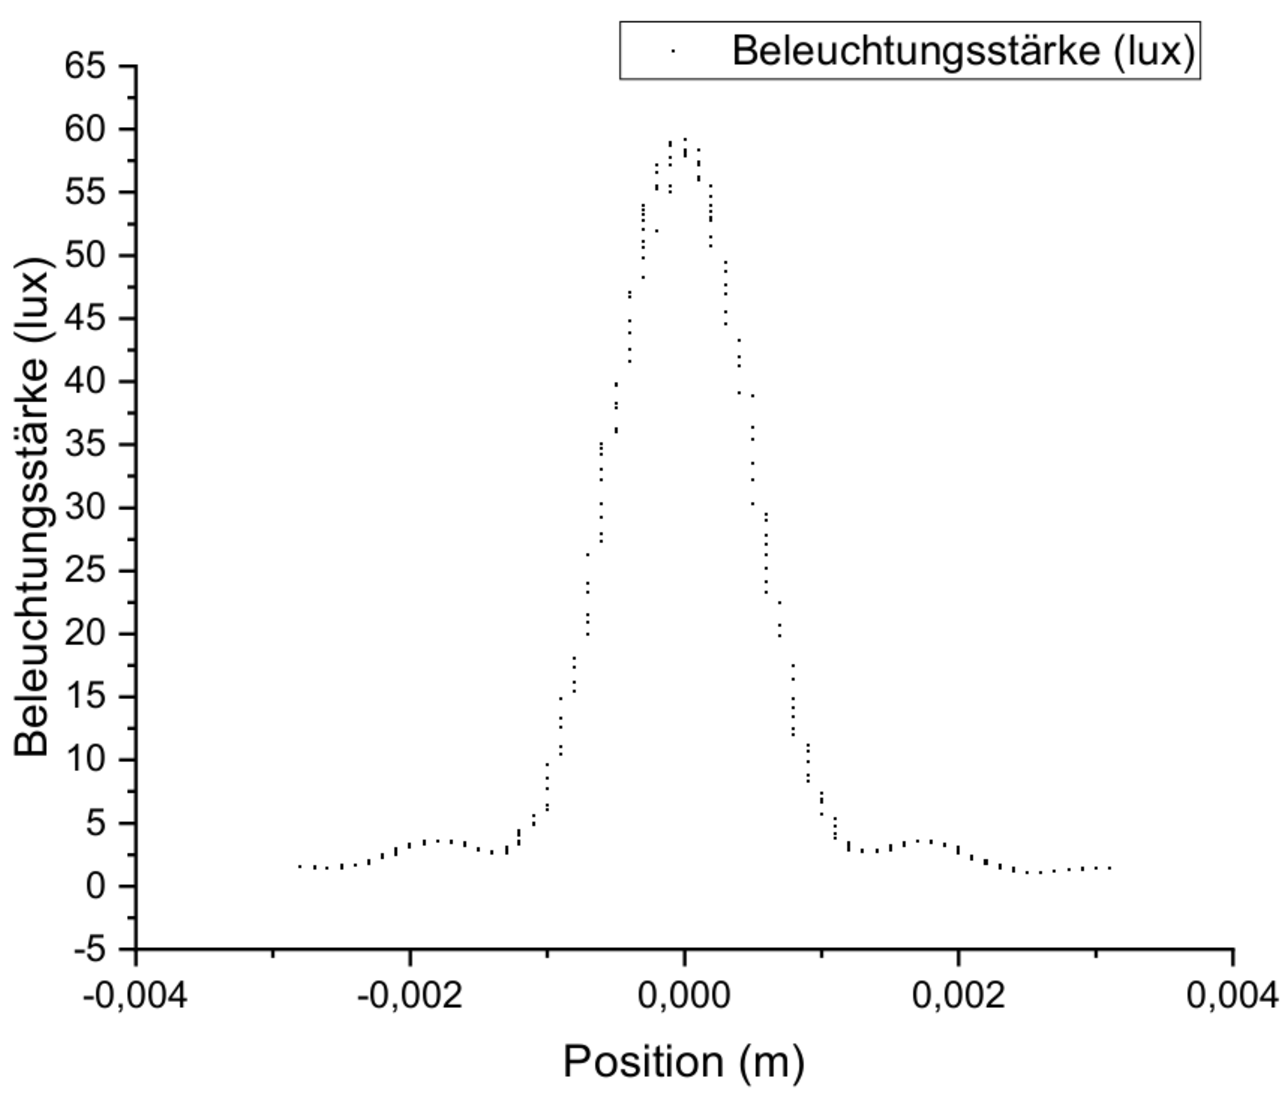
\includegraphics[width=1\linewidth]{Einzelspalt0-400mmZOOM}
			\caption{Extrema niedriger Ordnung}
		\end{subfigure}
		\caption{Intensitätsverteilung für einen Einzelspalt mit der Spaltbreite $b$ = \SI{0,4}{mm}.}
		\label{Einzelspalt0-400mm}
	\end{figure}

	\subsubsection{Intensitätsverteilung unterschiedlicher Mehrfachspalte} 
	In \cref{GitterGraphen} sind die Intensitätsverteilungen von Mehrfachspalten mit $N$ = 3,4,5 und 40 dargestellt. 
	\label{Maximaintensitäten}

	\begin{figure}[H]
		\centering
		\begin{subfigure}{.5\textwidth}
			\centering
			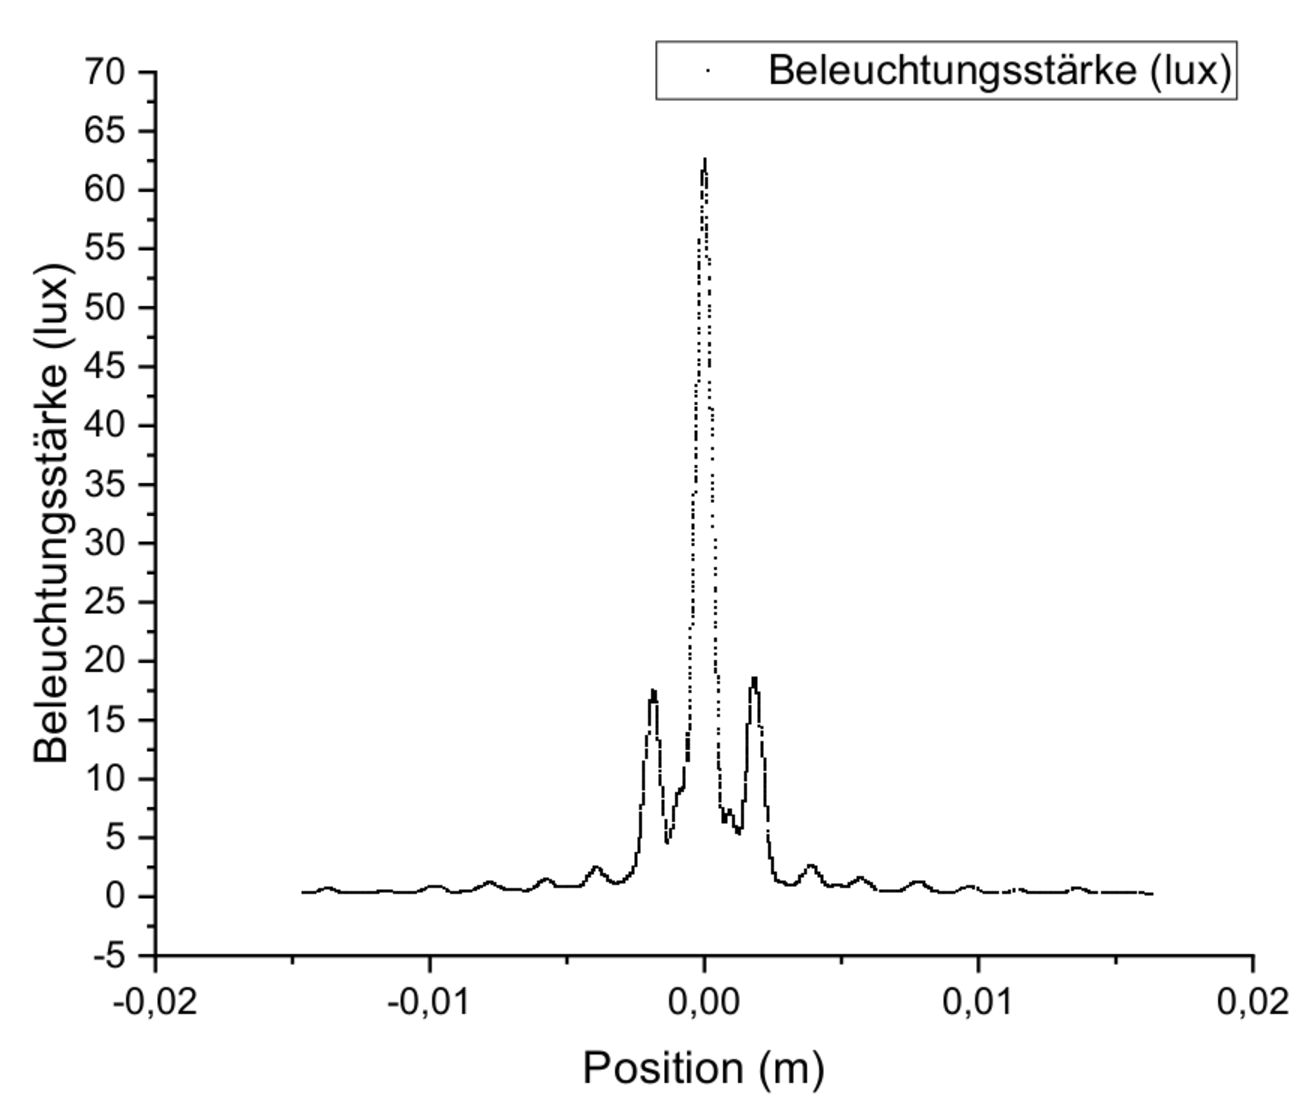
\includegraphics[width=1\linewidth]{GitterN3ZOOM}
			\caption{$N$=3}	
		\end{subfigure}%
		\begin{subfigure}{.5\textwidth}
			\centering
			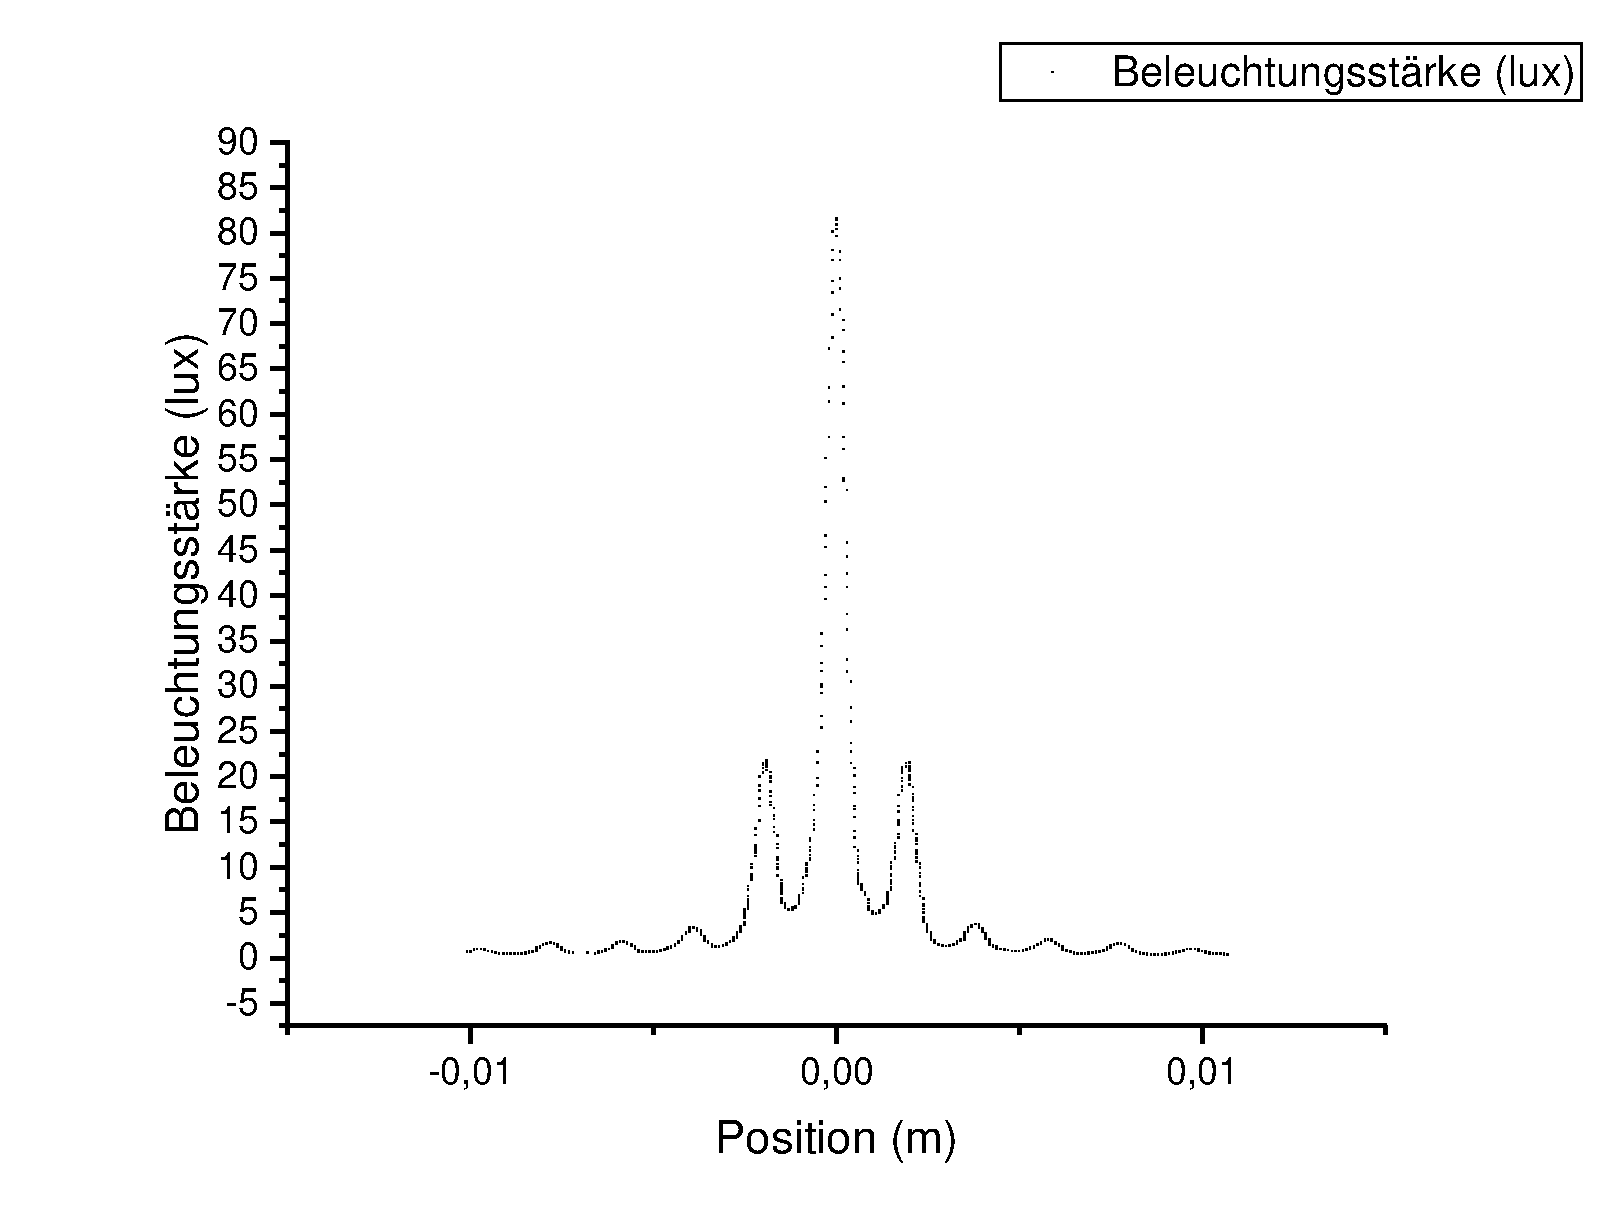
\includegraphics[width=1\linewidth]{GitterN4ZOOM}
			\caption{$N$=4}
		\end{subfigure}
		\begin{subfigure}{.5\textwidth}
			\centering
			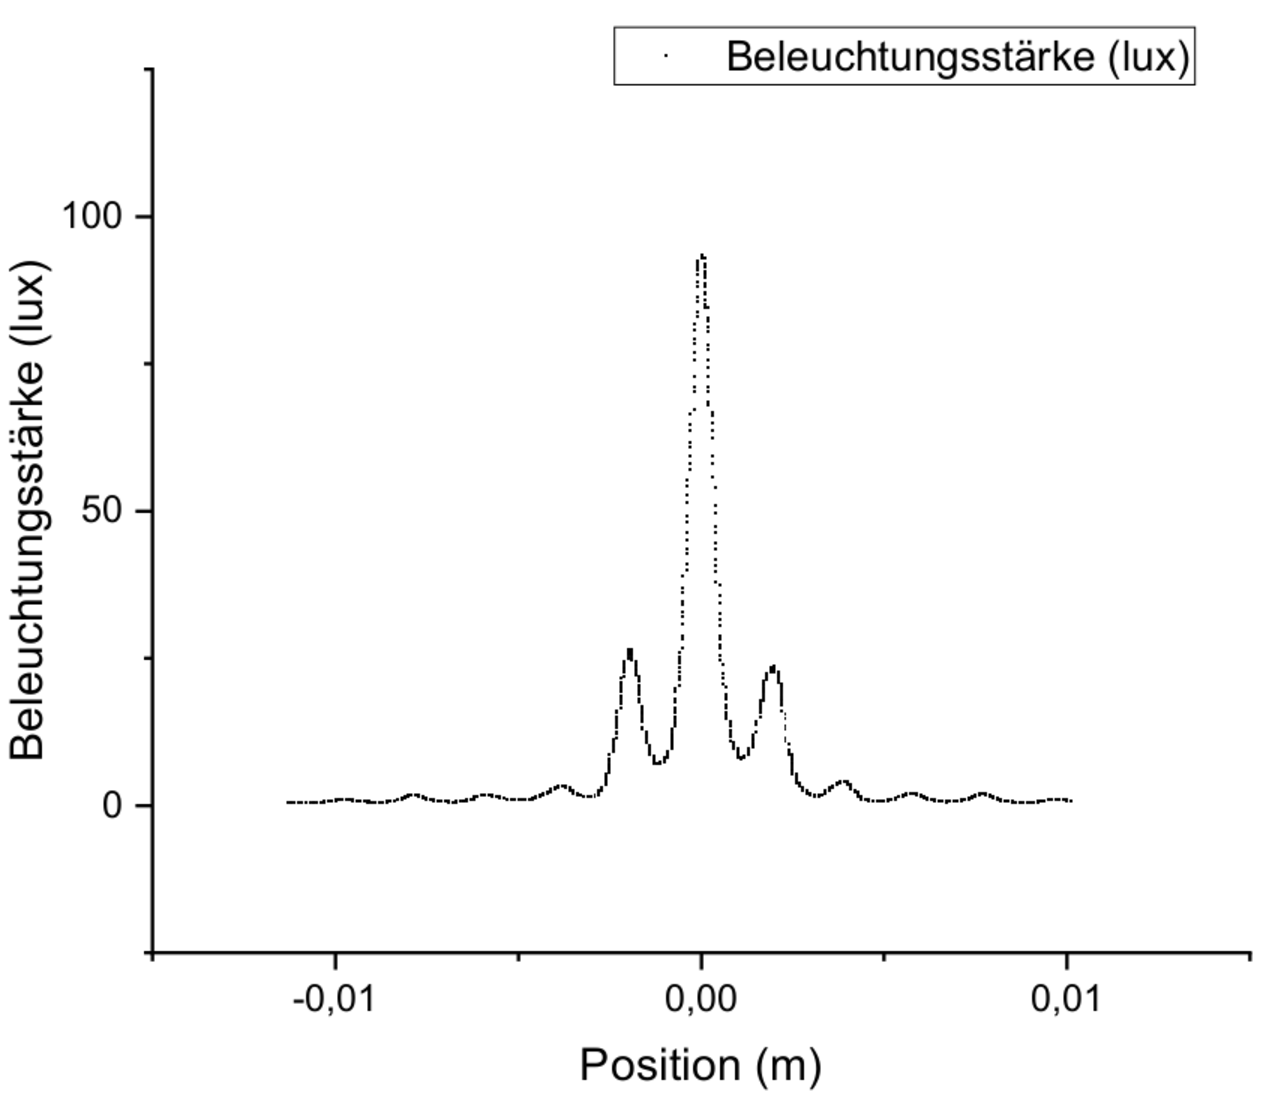
\includegraphics[width=1\linewidth]{GitterN5ZOOM}
			\caption{$N$=5}	
		\end{subfigure}%
		\begin{subfigure}{.5\textwidth}
			\centering
			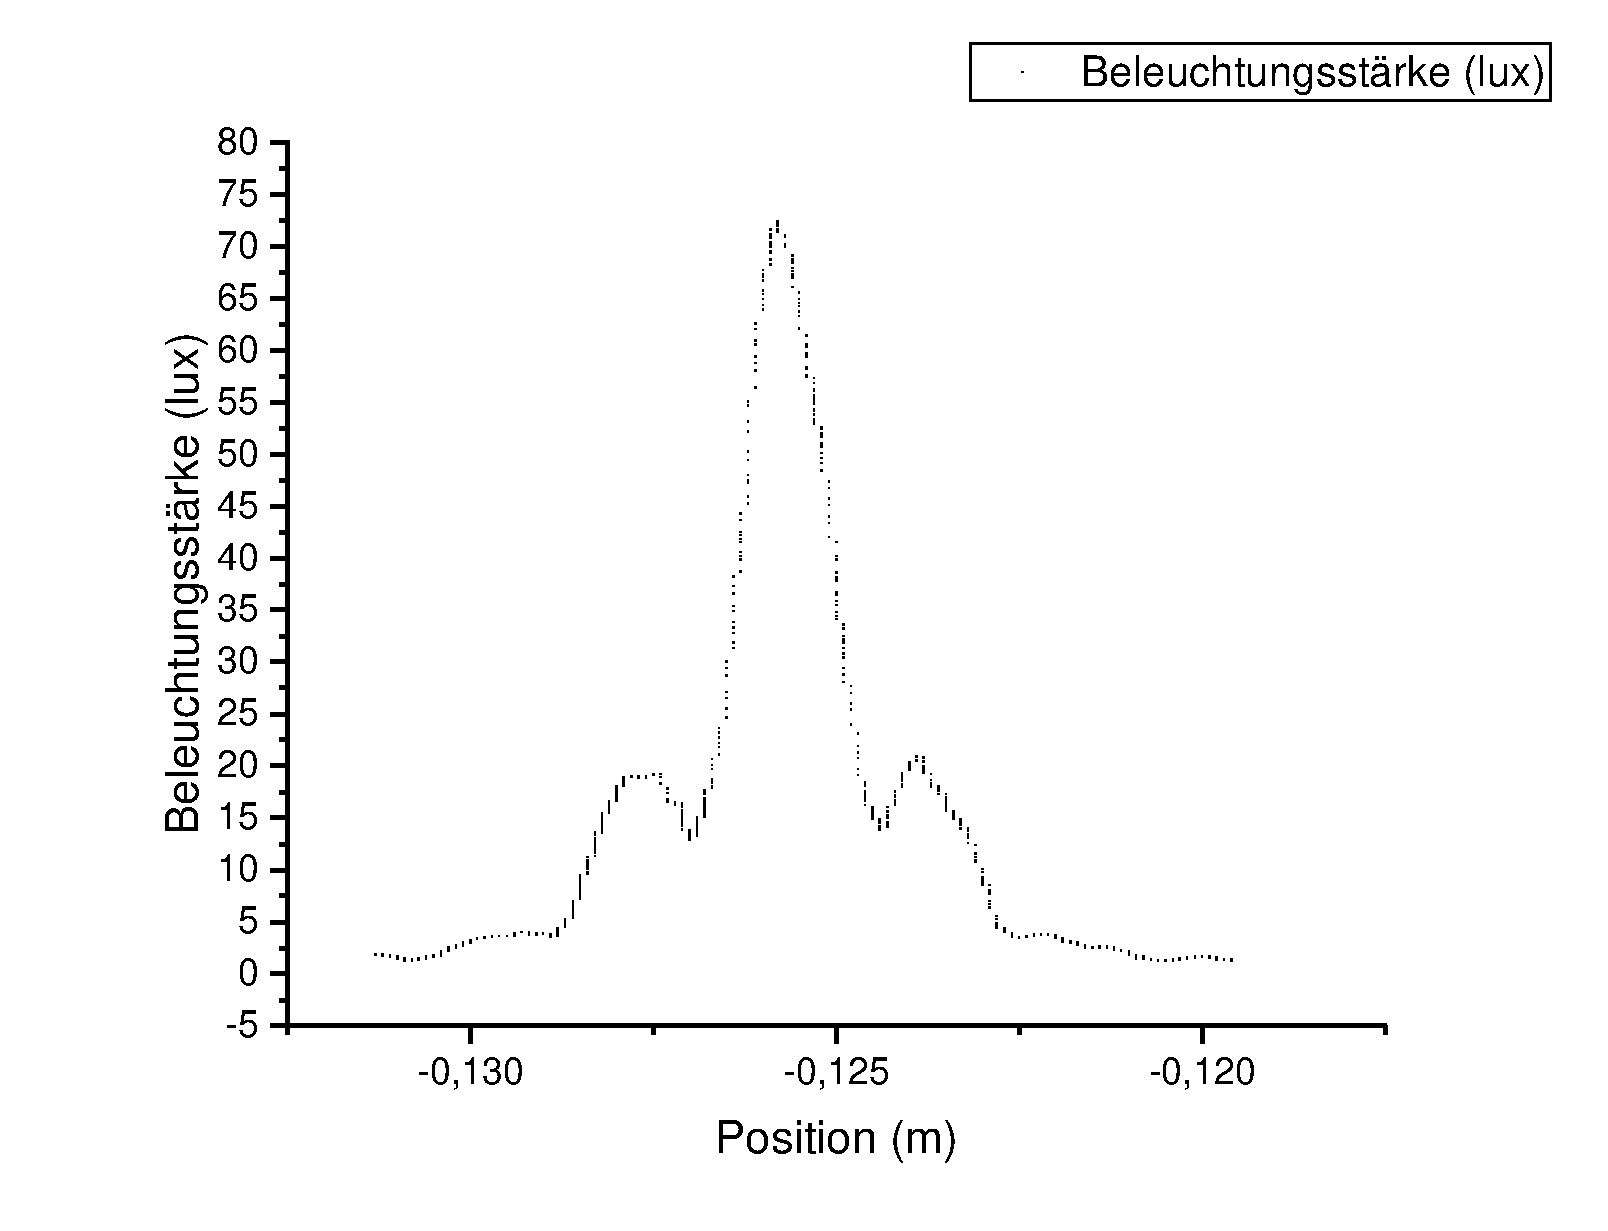
\includegraphics[width=1\linewidth]{GitterN40ZOOM}
			\caption{$N$=40}
		\end{subfigure}
		\caption{Intensitätsverteilungen verschiedener Mehrfachspalte  ($b$=\SI{0,15}{mm}, $g$=\SI{0,25}{mm}).}
		\label{GitterGraphen}
	\end{figure}

	

	
	Der Formfaktor wurde in der Einführung wie folgt definiert: 
	\begin{equation}
		I_m \propto \left[\frac{\sin(m\pi b/g)}{m\pi b/g}\right]^2
	\end{equation}
	Folglich ist
	\begin{equation}
		I_1/I_0 = \left[\frac{\sin(\pi b/g)}{\pi b/g}\right]^2
	\end{equation}
	und das Verhältnis b/g lässt sich bestimmen indem man $ \text{sinc}^2(\pi x)$ graphisch gleich dem Verhältnis $I_1/I_0$ setzt (unter der einschränkenden Voraussetzung $b/g<1$, da $\text{sinc}(x)$ sonst nicht umkehrbar ist).
	Die Intensitäten der ersten zwei Hauptmaxima und deren Halbwertsbreite sind in \cref{GitterTabelle} aufgeführt. 
	\begin{table}[H]
		\centering
		\begin{tabular}{ c | c | c | c }
			$N$ &  Intensität 0.HM & Intensität 1.HM & Halbwertsbreite\\ \hline
			3 & \SI{62,6 +- 0,5}{lux} & \SI{18,5 +- 0,5}{lux} & \SI{0,0006+- 0,00002}{m} \\
			4 & \SI{81,6 +- 0,5}{lux} & \SI{21,8 +- 0,5}{lux} & \SI{0,0006+- 0,00002}{m} \\
			5 & \SI{93,4 +- 0,5}{lux} & \SI{23,7 +- 0,5}{lux} & \SI{0,0008+- 0,00002}{m} \\
			40& \SI{72,3 +- 0,5}{lux} & \SI{18,9 +- 0,5}{lux} & \SI{0,0014+- 0,00002}{m} \\
		\end{tabular}
		\caption{Intensitäten und Halbwertsbreiten der Maxima unterschiedlicher Mehrfachspalte ($b$=\SI{0,15}{mm}, $g$ = \SI{0,25}{mm}).}
		\label{GitterTabelle} 
	\end{table}
	
	Ein Hauptmaximum erster Ordnung erfüllt die Bedingung
	\begin{equation}
		\sin(\vartheta) = \pm \frac{\lambda}{g}
	\end{equation}
	somit lässt sich aus der Position des Hauptmaximums mit \cref{dreieck} und der Wellenlänge $\lambda$ die Gitterkonstante $g$ bestimmen.
	\begin{equation}
		g = \lambda\sqrt{(d/x)^2 + 1}
	\end{equation}
	\begin{equation}
		u(g) = g\sqrt{\left(\frac{u(\lambda)}{\lambda}\right)^2 + \left( \frac{u(d)d}{d^2 + x^2}\right)^2 + \left(\frac{u(x)d^2}{x(d^2 + x^2)}\right)^2}
	\end{equation}
	Die Positions des ersten Hauptmaximums war unabhängig von der Anzahl der Spalte $|x|$= \SI{0,0021+- 0,0001}{m} und mit einem $\lambda$ von \SI{663+-11}{nm} und $d$ = \SI{0,78 +-0,009}{m} ergibts sich $g$ =\SI{0,246+- 0,013}{mm}.
	Aus dem zuvor ermittelten Verhältnis von $b/g$ lässt sich nun auch $b$ bestimmen. Die jeweiligen Werte sind in \cref{FormTabelle} aufgelistet.
	\begin{table}[H]
		\centering
		\begin{tabular}{ c | c | c | c | c }
			$N$ &  3 & 4 & 5 & 40\\ \hline
			$I_1/I_0$ & \SI{0,29+-0,008}{} & \SI{0,27+-0,006}{} & \SI{0,25+-0,005}{} & \SI{0,26+-0,007}{} \\
			$b/g$& \SI{0,57+-0,005}{} & \SI{0,59+-0,005}{} & \SI{0,60+-0,005}{} & \SI{0,60+-0,005}{} \\
			$g$& \SI{0,246+- 0,013}{mm} & \SI{0,246+- 0,013}{mm} & \SI{0,246+- 0,013}{mm} & \SI{0,246+- 0,013}{mm} \\
			$b$ & \SI{0,140+- 0,007}{mm} & \SI{0,145+- 0,008}{mm} & \SI{0,147+- 0,008}{mm}& \SI{0,147+- 0,008}{mm}\\
		\end{tabular}
		\caption{Verhältnis zwischen erstem und nulltem Hauptmaximum. }
		\label{FormTabelle} 
	\end{table}

	\subsection{Diskussion}
	\subsubsection{Wellenlänge des Lasers}
	Aus den Extrema der Einzelspalte wurde eine Wellenlänge des Lasers von \SI{663\pm 11}{nm} bestimmt.
	Dies deckt sich mit der Angabe von \SI{630}{\nano \meter} bis \SI{680}{\nano \meter} auf dem Laser.
	
	\subsubsection{Vergleich von Einzelspalt und Doppelspalt}
	Wenn man die Intensitätsverteilung eines Einzelspalts mit $b=\SI{0,15}{mm}$ (vgl. \cref{Einzelspalt0-150mm}) mit einem Doppelspalt mit gleicher Spaltbreite vergleicht (vgl. \cref{Doppelspalt0-15mm}), lässt sich erkennen, dass die Maxima höherer Ordnung des Doppelspalts eine deutlich höhere Intensität verglichen mit dem Maxima nullter Ordnung haben als beim Einzelspalt.
	Außerdem liegen die Maxima bei unterschiedlichen Positionen, was der Theorie entspricht, da sie von $g$ abhängig sind.
	Dass die Einhüllende des Doppelspalts der Intensitätsverteilung des Einzelspalts entspricht, lässt sich aus den Messungen nicht hinreichend eindeutig ablesen.
	
	\begin{figure}[H]
		\centering
		\begin{subfigure}{.5\textwidth}
			\centering
			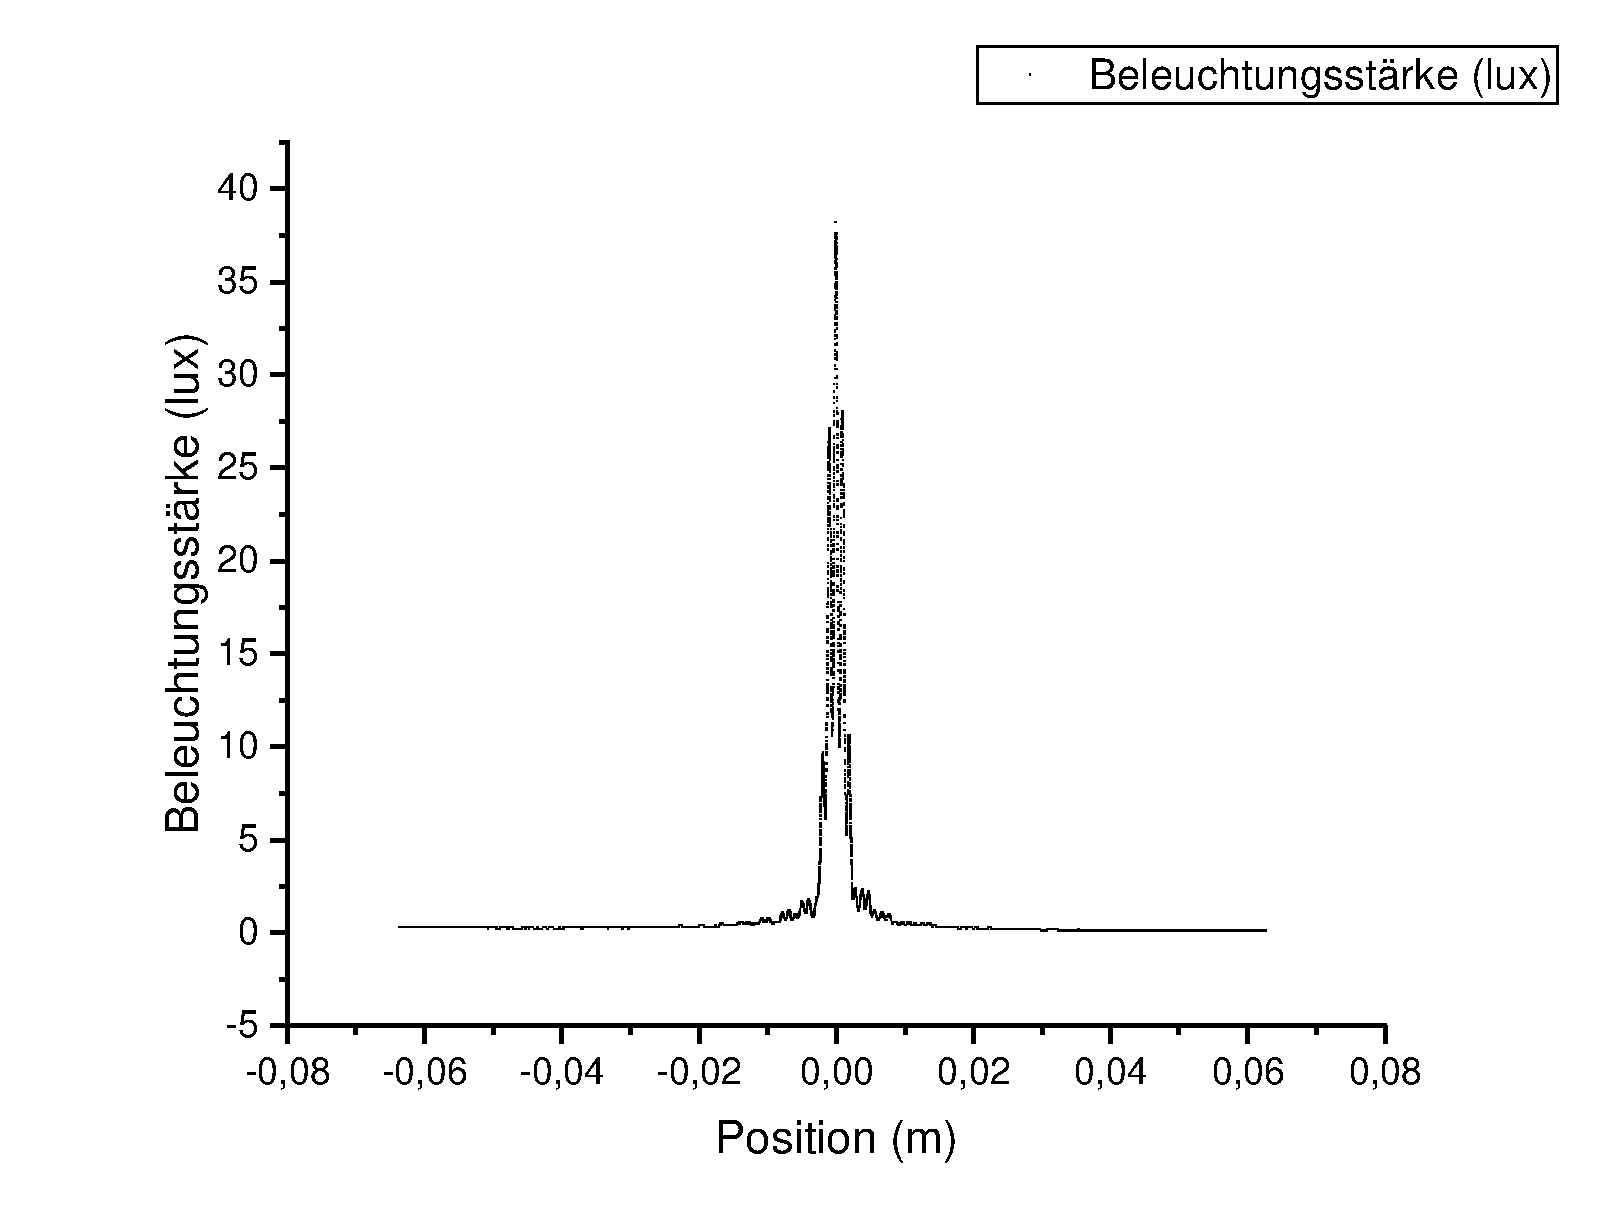
\includegraphics[width=1\linewidth]{Doppelspaltb0-15mmg0-5mmNOZOOM}
			\caption{Gesamte Messung}	
		\end{subfigure}%
		\begin{subfigure}{.5\textwidth}
			\centering
			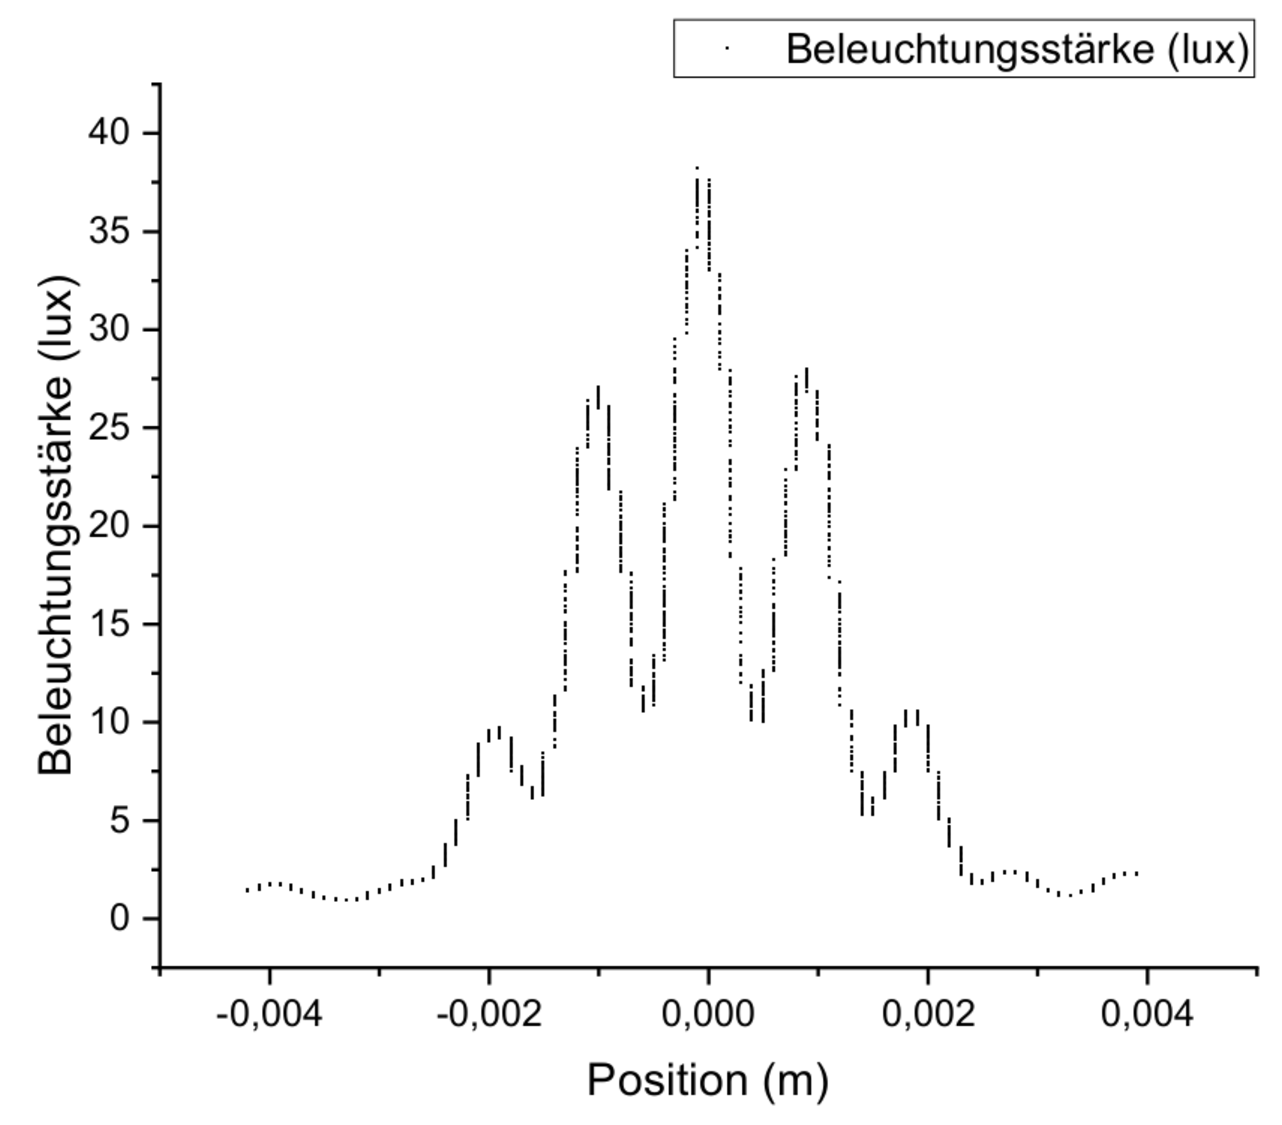
\includegraphics[width=1\linewidth]{Doppelspaltb0-15mmg0-5mm}
			\caption{Extrema niedriger Ordnung}
		\end{subfigure}
		\caption{Intensitätsverteilung für einen Doppelspalt mit der Spaltbreite $b = \SI{0,15}{mm}$ und $g = \SI{0,5}{mm} $ .}
		\label{Doppelspalt0-15mm}
	\end{figure}
	
	\subsubsection{Vergleich verschiedener Doppelspalte}
	In \cref{Doppelspaltvergleich} sind Doppelspalte verschiedener Spaltbreiten und Spaltabstände dargestellt.
	Dabei lässt sich erkennen, dass bei höherem Spaltabstand die Maxima näher zusammen liegen.
	Dies bestätigt die Theorie, da die Maxima bei Vielfachen von $\sin \vartheta = \lambda /g $ liegen sollten. \label{Doppelspalttheo}
	Für die Spaltbreite lässt sich ein eindeutiger Zusammenhang zwischen steigender Spaltbreite und sinkender relativer Intensität der Maxima höherer Ordnung (im Vergleich zum Maximum nullter Ordnung) erkennen.
	Dies ergibt sich daraus, dass bei höherer Spaltbreite die Beugungseffekte abnehmen und der Lichtstrahl eher wie in der geometrischen Optik verhält.
	
	\begin{figure}[H]
		\centering
		\begin{subfigure}{.5\textwidth}
			\centering
			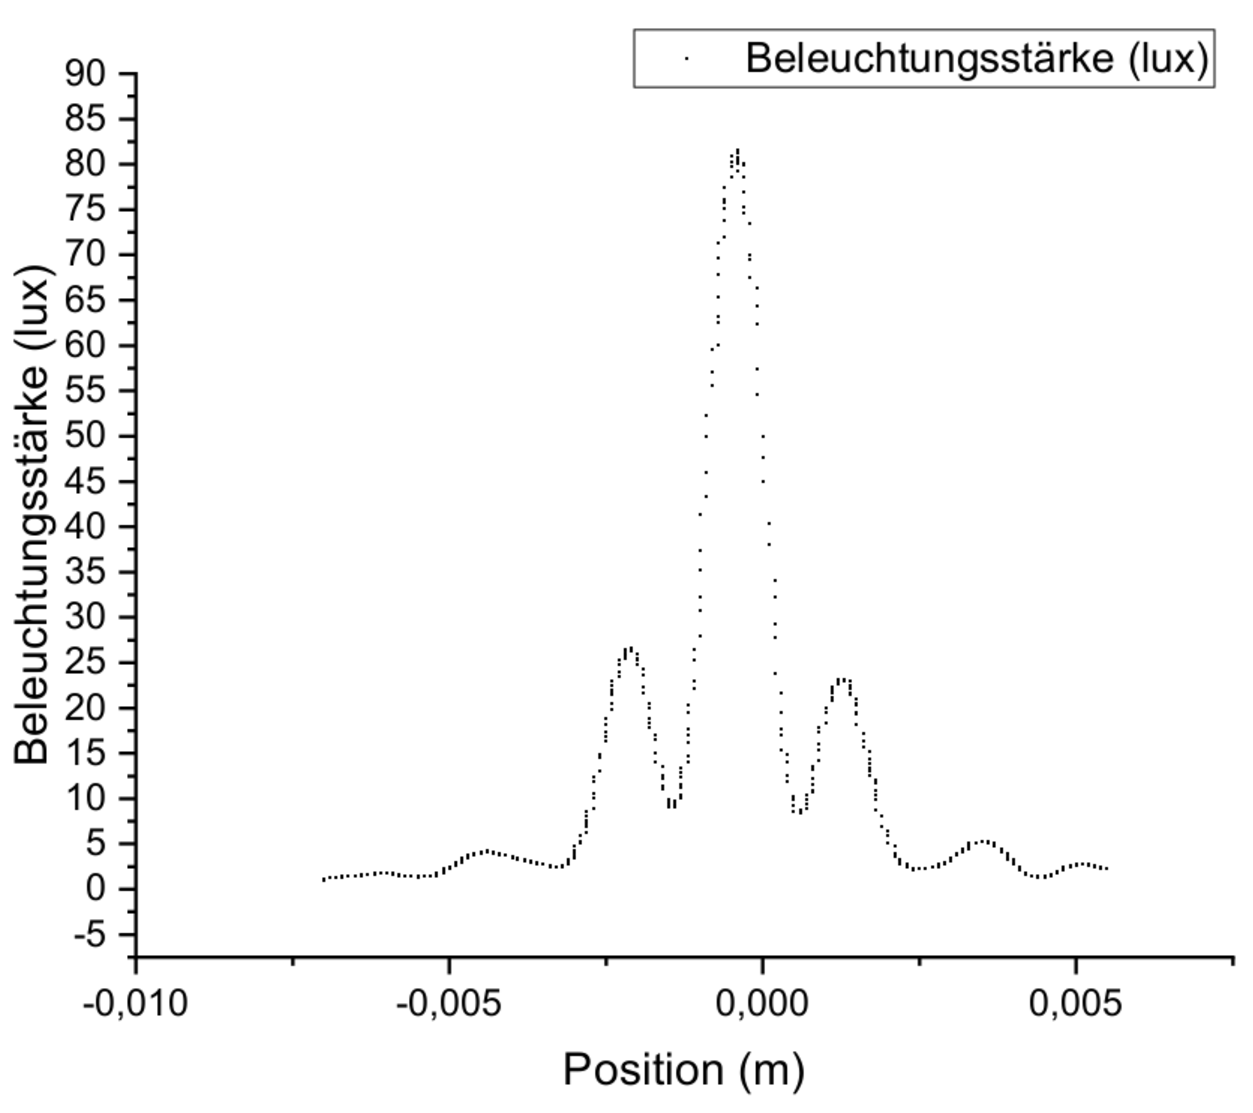
\includegraphics[width=1\linewidth]{Doppelspaltb0-15mmg0-25mm.pdf}
			\caption{$b=\SI{0,15}{mm}$, $ g=\SI{0,25}{mm}$}	
		\end{subfigure}%
		\begin{subfigure}{.5\textwidth}
			\centering
			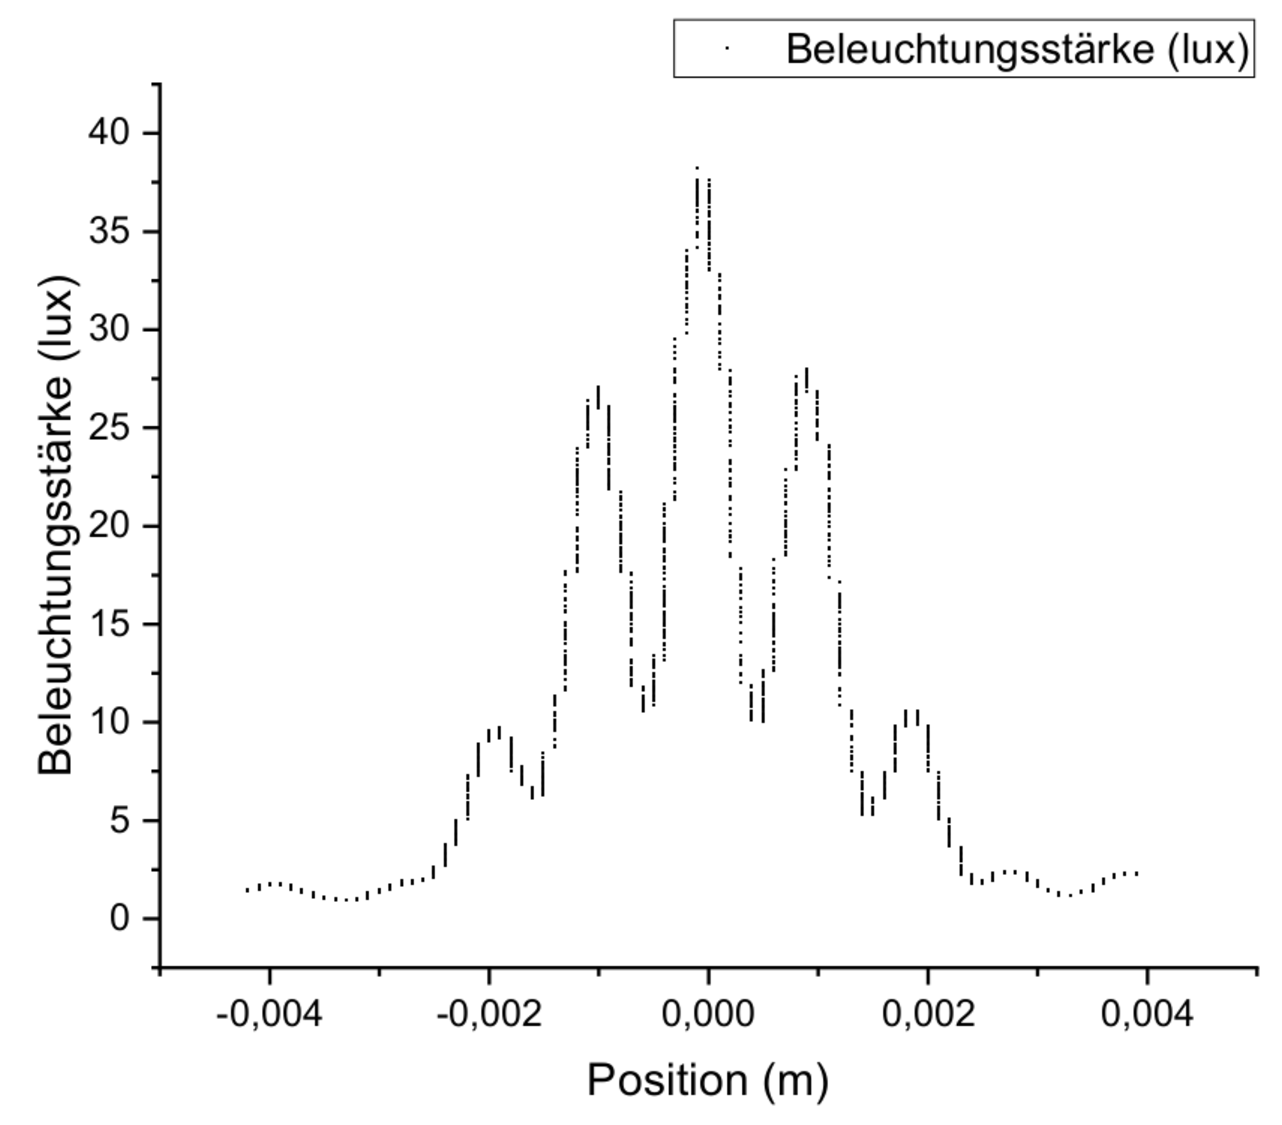
\includegraphics[width=1\linewidth]{Doppelspaltb0-15mmg0-5mm.pdf}
			\caption{$b=\SI{0,15}{mm}$, $ g=\SI{0,5}{mm}$}
		\end{subfigure}
		\begin{subfigure}{.5\textwidth}
			\centering
			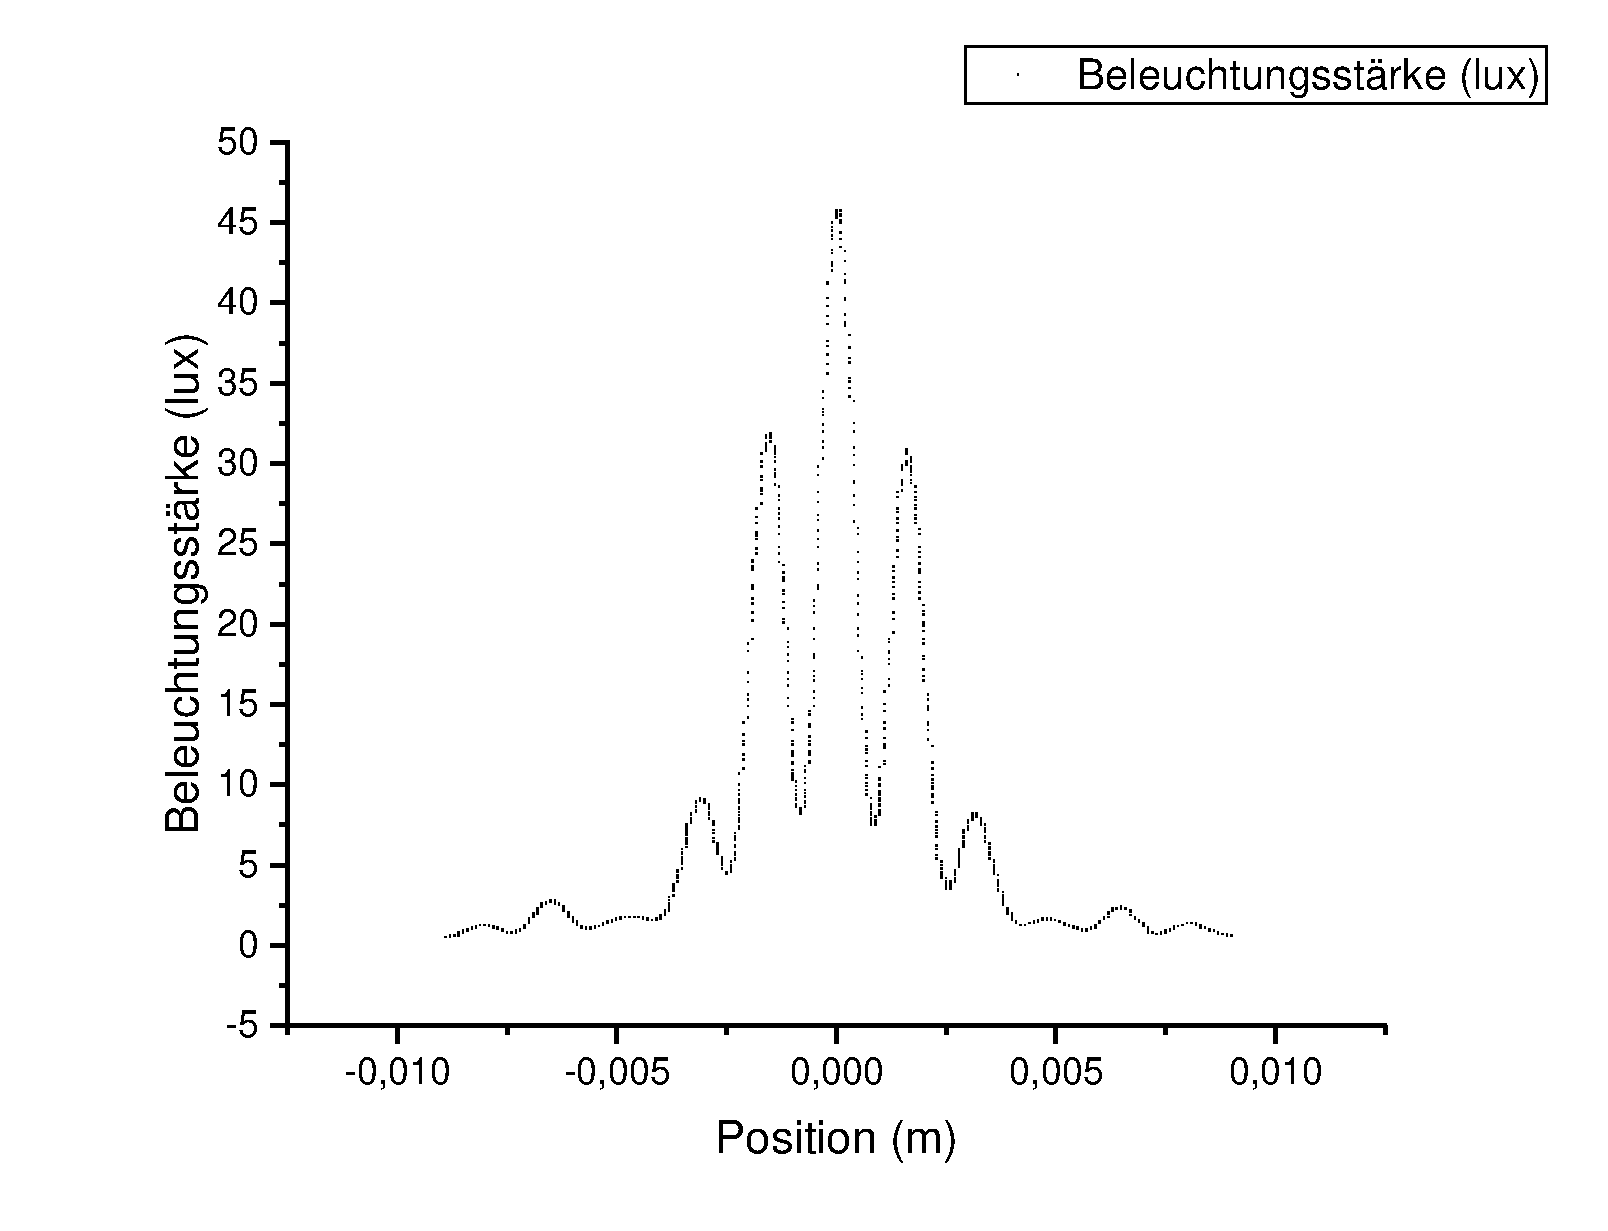
\includegraphics[width=1\linewidth]{Doppelspaltb0-10mmg0-30mm}
			\caption{$b=\SI{0,1}{mm}$, $ g=\SI{0,3}{mm}$}	
		\end{subfigure}%
		\begin{subfigure}{.5\textwidth}
			\centering
			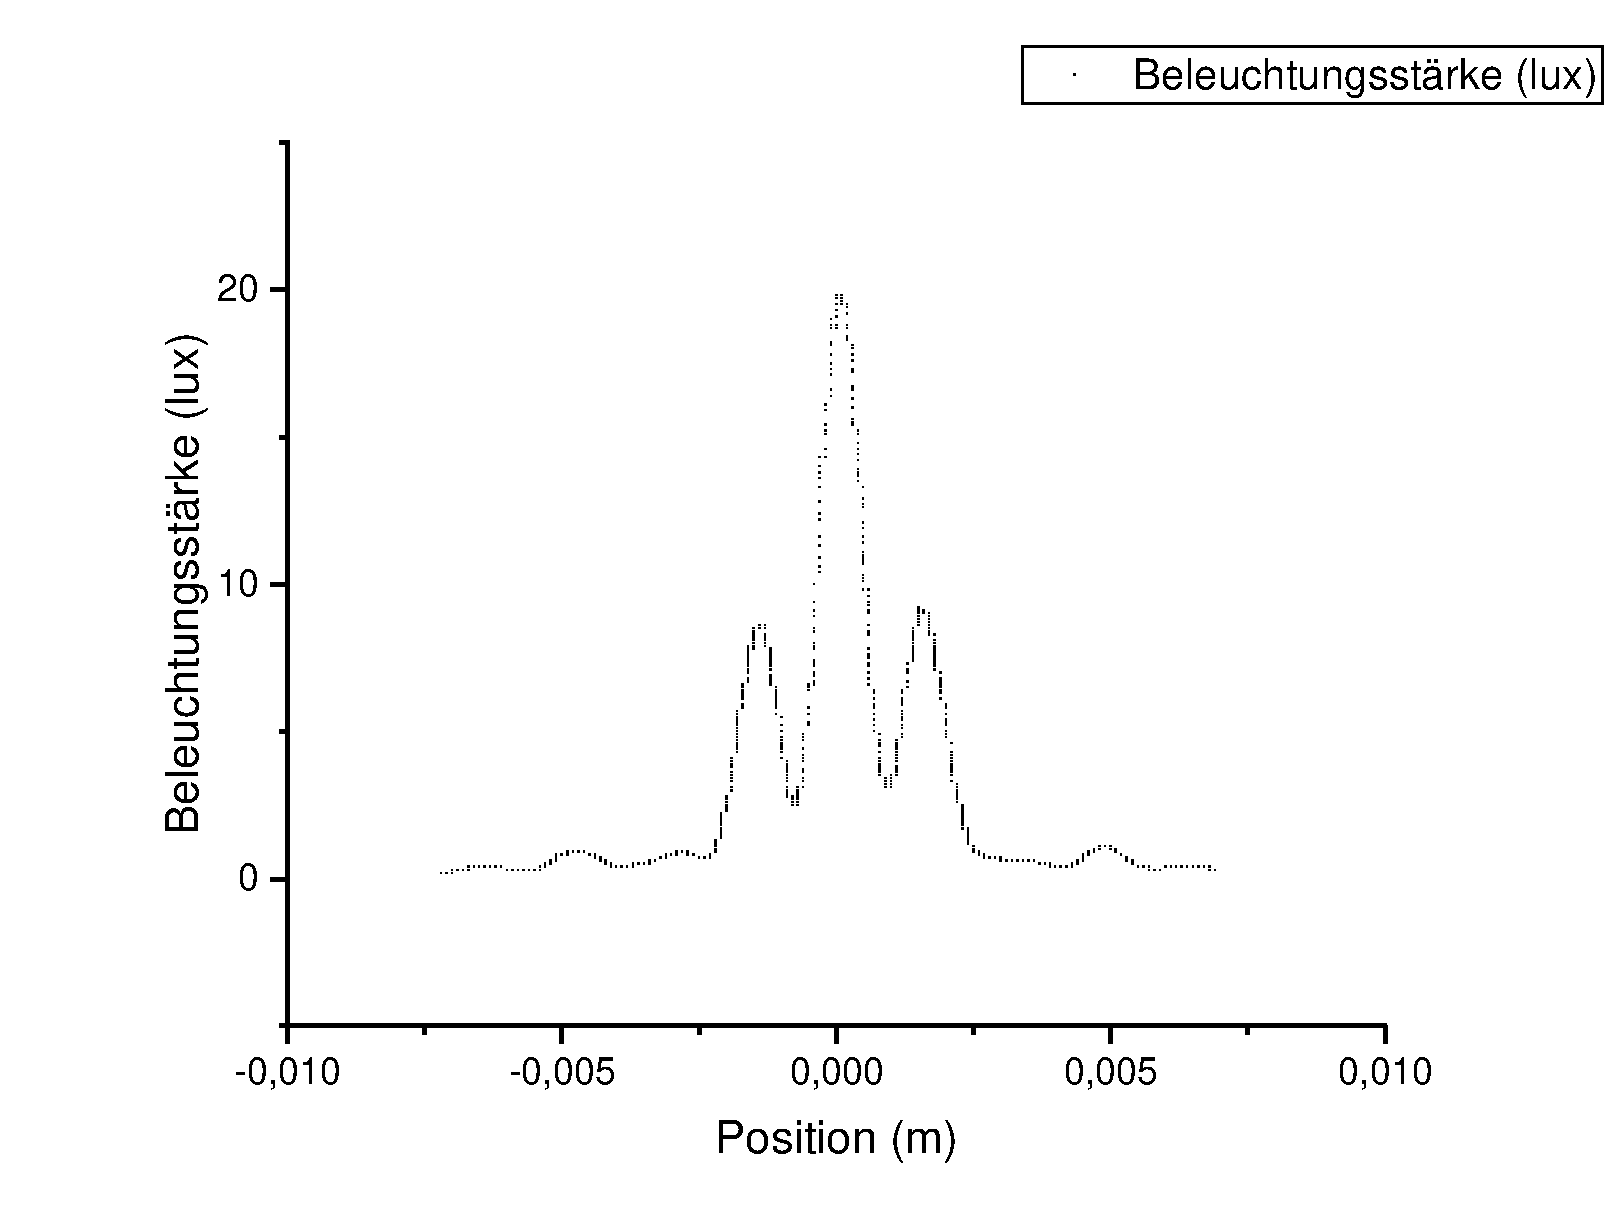
\includegraphics[width=1\linewidth]{Doppelspaltb0-15mmg0-30mm}
			\caption{$b=\SI{0,15}{mm}$, $ g=\SI{0,3}{mm}$}
		\end{subfigure}
		\caption{Intensitätsverteilungen verschiedener Doppelspalte.}
		\label{Doppelspaltvergleich}
	\end{figure}
	
	\subsubsection{Intensitätsverteilung unterschiedlicher Mehrfachspalte}
	In \cref{HMGitterGRaph} sind die Intensitäten der Maxima verschiedener Mehrfachspalte gegen die Zahl der Spalte aufgetragen.
	Nicht betrachtet wird hier das Gitter mit 40 Spalten, da dieses vom Laser nicht über die gesamte Breite ausgeleuchtet wird und somit nicht mit den Intensitäten der anderen Gitter verglichen werden kann.
	Die Intensitäten der Hauptmaxima sollten der Einführung zufolge quadratisch von der Anzahl der Spalte abhängen, während die Messung eher einen linearen Zusammenhang vermuten lässt.
	Dies könnte damit zusammen hängen, dass, wenn man einen im Durchschnitt annähernd kreisförmigen Laserstrahl annimmt, die Spalte am Rand zu einem geringeren Anteil durchleuchtet werden als die Spalte in der Mitte und nicht sichergestellt werden kann, dass die Photodiode immer exakt auf der Höhe des Laserstrahls misst.
	Auch dass die Spaltanordnung exakt mittig vom Laserstrahl getroffen wird, kann mit dieser Versuchsanordnung nicht sichergestellt werden. %TODO bitte einmal confirmen
	
	\begin{figure}[H]
		\centering
		\begin{subfigure}{.5\textwidth}
			\centering
			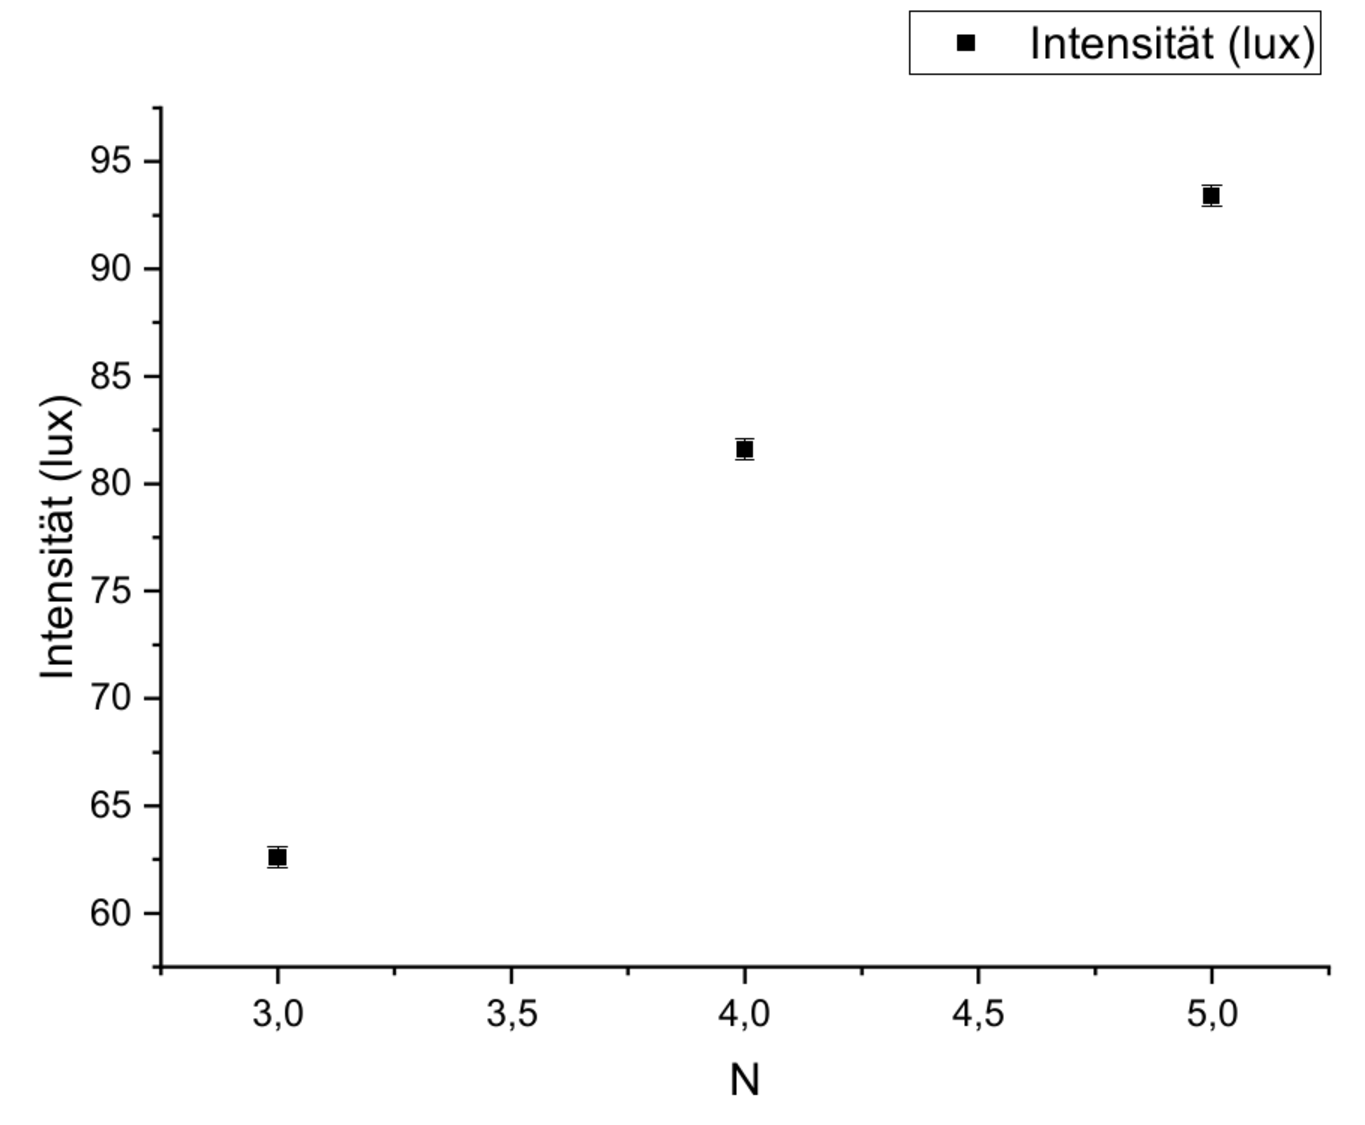
\includegraphics[width=1\linewidth]{0HMGitter}
			\caption{Nullte Hauptmaxima}	
		\end{subfigure}%
		\begin{subfigure}{.5\textwidth}
			\centering
			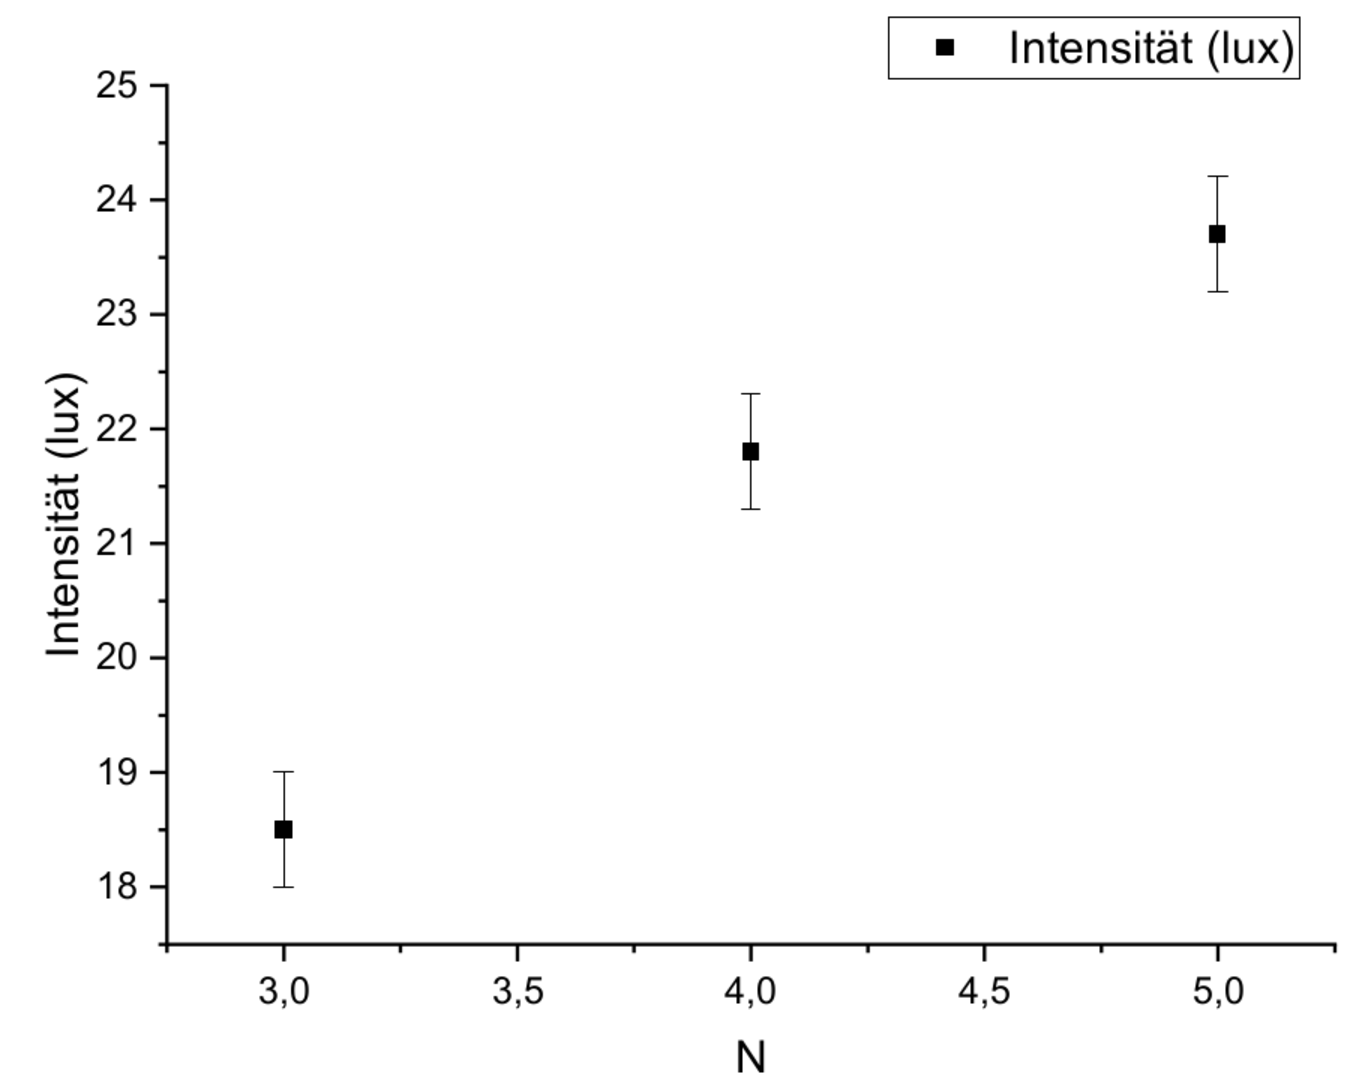
\includegraphics[width=1\linewidth]{1HMGitter}
			\caption{Erste Hauptmaxima}
		\end{subfigure}
		\label{HMGitterGRaph}
		\caption{Intensitäten der Maxima unterschiedlicher Mehrfachspalte ($b$ = \SI{0,15}{mm}, $g$=\SI{0,25}{mm}).}
	\end{figure}

	Die Halbwertsbreite hat sich in der Messung mit der Anzahl der Spalte nur geringfügig geändert (wenn man mit demselben Argument wie oben $N=40$ nicht betrachtet).
	Für eine präzisere Aussage über diesen Zusammenhang benötigt man eine bessere Winkelauflösung.
	\subsubsection{Nebenmaxima eines Vierfachspalts}
	Wie man in \cref{GitterGraphen} erkennen kann, konnten bei diesem Versuchsaufbau die Nebenmaxima des Vierfachspalts nicht aufgelöst werden.
	Dies kann einerseits an dem mangelnden Winkelauflösungsvermögen der Versuchsanordnung durch das Messrad liegen, aber auch an der mangelnden Genauigkeit des Messprogramms beim Exportieren der Messergebnisse.
	
	%TODO "Wo erwarten Sie die (Haupt)Maxima und Minima? "
	

	
	\section{Schlussfolgerung}
	Insgesamt gesehen konnten einige aber nicht alle der Hypothesen bestätigt werden.
	Die Wellenlänge des Lasers konnte gemessen werden und bestätigt mit einem Wert von \SI{663\pm 11}{nm} die Angabe auf dem Gerät.
	Für eine bessere Überprüfbarkeit wäre jedoch eine Angabe in der Form $\lambda = x\pm a$ im wissenschaftlichen Kontext geeigneter als die Angabe des Bereichs von \SI{630}{\nano \meter} bis \SI{680}{\nano \meter}, da hier nicht klar ist, ob dies eine Angabe gemäß des Guide to the Expression of Uncertainty in Measurement ist.
	
	Die Intensitätsverteilung des Einzelspalts verläuft wie erwartet wie eine quadrierte sinc-Funktion.
	Dass die einhüllende Funktion der Intensitätsverteilung eines Doppelspalts der Intensitätsverteilung eines Einzelspalts mit gleicher Spaltbreite entspricht, konnte nicht eindeutig bestätigt werden.
	Aber die Auswirkungen einer Änderung von Spaltabstand und Spaltbreite eines Doppelspalts auf das Intensitätsbild konnten der Theorie entsprechend gemessen werden.
	Auch der Anstieg der Intensität der Hauptmaxima mit der Anzahl der Spalte konnte für die vom Laser vollständig ausgeleuchteten Spaltanzahlen bestätigt werden sowie die Gitterstruktur bestimmt werden.
	Der quadratische Zusammenhang zwischen Zahl der Spalte eines Gitters und Intensität der Hauptmaxima konnte nicht gezeigt werden.
	
	Im Allgemeinen hätten sich präzisere Aussagen machen lassen, wenn dass Messprogramm beim Exportieren der Werte diese nicht nachträglich runden würde.
	Auch ein größerer Abstand zwischen Beugungsanordnung und Photodiode würde die Winkelauflösung erhöhen.
	
	%TODO Quellen zitieren, Websiten mit Zugriffsdatum
	%TODO Verweise auf das Laborbuch (sind erlaubt)
	%TODO Tabelle + Bilder mit Beschriftung
	\printbibliography
\end{document}
